\documentclass[conference]{IEEEtran}
\usepackage{amsmath,amssymb,booktabs,array,enumitem,algorithm,algpseudocode,microtype,graphicx,pgfplots,placeins}
\usepackage[hidelinks]{hyperref}
\hypersetup{pdftitle={Lightweight Trap-Based Free-Rider Detection and Mitigation in Federated Learning},pdfauthor={Aashnan Rahman},pdfkeywords={federated learning,free-rider detection,robust statistics}}
\pgfplotsset{compat=1.18}
\usepgfplotslibrary{groupplots,fillbetween}
\definecolor{honestblue}{HTML}{2878A5}
\definecolor{riderorange}{HTML}{D66B27}
\providecommand*{\algorithmautorefname}{Algorithm}
\makeatletter
\setlength{\@fptop}{0pt}
\setlength{\@fpsep}{14pt}
\setlength{\@fpbot}{0pt plus 1fil}
\setlength{\@dblfptop}{0pt}
\setlength{\@dblfpsep}{14pt}
\setlength{\@dblfpbot}{0pt plus 1fil}
\makeatother
\newcommand{\StudyRuns}{32}
\newcommand{\StudyTP}{1120}
\newcommand{\StudyFP}{0}
\newcommand{\StudyFN}{0}
\newcommand{\StudyHonest}{2080}
\newcommand{\StudyQuarantined}{11}
\newcommand{\StudyQuarantineRounds}{220}
\newcommand{\StudyCandidates}{296}

\title{Lightweight Trap-Based Free-Rider Detection and Mitigation in Federated Learning}
\author{\IEEEauthorblockN{Aashnan Rahman}
\IEEEauthorblockA{Department of Computer Science and Engineering\\
Islamic University of Technology\\MSc Thesis}}
\begin{document}
\maketitle
\begin{tikzpicture}[remember picture,overlay]
\node[anchor=north east,font=\footnotesize] at ([xshift=-0.55in,yshift=-0.32in]current page.north east) {Last updated on 18 October 2026};
\end{tikzpicture}

\begin{abstract}
Federated learning relies on participants performing useful local optimization,
but free riders can consume the shared model while submitting unchanged or
fabricated responses. Detecting such behavior is difficult when honest clients
have heterogeneous data and naturally different update statistics. This paper
investigates a server-side challenge protocol that compares responses to
undisclosed perturbations of the same model. Robust update-norm and tensor-profile
measurements first nominate anomalous clients; separate geometric separation
tests and repeated fresh evidence authorize removal. Component-specific memory
retains strong evidence across ambiguous cycles, while bounded quarantine
prevents weak suspicion from causing indefinite exclusion. The method requires
no auxiliary detector training, client-reported loss, or attack-specific history
reconstruction. We evaluate \StudyRuns{} completed 100-round runs covering four
fabrication strategies, MNIST and CIFAR-10, IID and Dirichlet non-IID data, and
30\% and 40\% free riders. All \StudyTP{} free-rider client-cases are removed,
with no permanent removal among \StudyHonest{} honest client-cases. Complete
removal occurs at round 30 except for non-IID CIFAR-10 history averaging, which
requires rounds 60 and 80. However, \StudyQuarantined{} honest client-cases
experience temporary quarantine, and substantial weak candidate populations
remain. The findings support the approach under the evaluated setting, not a
universal detection guarantee: the study uses one development seed and does not
evaluate adaptive adversaries or secure aggregation.
\end{abstract}
\begin{IEEEkeywords}
federated learning, free-rider detection, hidden challenges, robust statistics,
non-IID data, client auditing
\end{IEEEkeywords}

\section{Introduction}
Federated learning (FL) allows multiple participants to build a shared model
without collecting their raw training data at a single server. In each round,
the server distributes a model, clients optimize it using local examples, and
the server combines their returned contributions. Federated Averaging (FedAvg)
provides a foundational implementation of this process~\cite{mcmahan2017communication}.
Its collaborative benefit depends on local computation actually taking place:
a returned parameter vector is observable, but the work that produced it is not.

A participant may lack suitable data, face limited computing resources, or
prefer to save computation while retaining access to the jointly trained model.
Such a participant can return the received model, construct a random update, or
imitate the trajectory of previously received models. These free-rider behaviors
have been studied separately from deliberate model poisoning~\cite{lin2019freeriders,fraboni2021freerider}.
Their central harm is omitted useful contribution and an unequal allocation of
training effort; fabricated responses can also interfere with aggregation.
The counterfactual value of the missing honest update is not directly observable.

The detection problem is therefore not simply to identify the smallest update.
An honest client can have a small update because its local objective is nearly
satisfied, while another honest client can have an unusual layer profile because
its label distribution differs from its peers. Conversely, a free rider can add
noise to avoid exact equality or imitate geometric properties of training
updates~\cite{zhu2021advanced}. A useful defense needs evidence stronger than one
unusual norm, but should not require access to private datasets, trusted
client-reported metrics, or a separately trained anomaly model.

We examine a challenge-based alternative. The server occasionally sends a
scale-aware perturbation of a frozen global model and compares only responses
to that same challenge. These controlled inputs can make differences between
genuine optimization and the evaluated fabrication strategies observable.
However, a statistical split is not sufficient to establish misconduct. We
separate weak nomination, strong geometric evidence, temporary quarantine, and
permanent removal, and require repeated fresh evidence from the same component.

The principal contributions are as follows:
\begin{itemize}[leftmargin=*,nosep]
\item \textbf{Server-observable challenge protocol.} The method uses attributable
model responses and server-generated traps, without client loss, sample-count
claims, resource telemetry, or attacker labels as decision inputs.
\item \textbf{Separation-gated confirmation.} Robust scalar screening nominates
clients, but removal requires same-component evidence on two traps in distinct
cycles. Low-norm evidence must pass a strict full-peer separation test rather
than a compactness test alone.
\item \textbf{Evidence memory with bounded disruption.} Strong evidence can
survive ambiguous cycles, but stored evidence alone cannot renew quarantine.
Clean cycles clear memory, and unconfirmed exclusion has a bounded review period.
\item \textbf{Complete outcome accounting.} We report all 32 scheduled runs,
including removal timing, model accuracy, honest candidate flags, temporary
quarantine, withheld training responses, and whole-process execution cost.
\end{itemize}

The remainder of the paper reviews prior work, states the threat model, describes
the method, and presents the completed experiments. Result analysis distinguishes
successful removal from screening quality and utility. Security analysis then
examines the protocol's invariants, evasion risks, privacy requirements, and
limits of the evidence. Detailed per-run results and reproducibility information
are provided in the appendices.

\section{Literature Review}
\subsection{Free-Rider Attacks and Observable Update Geometry}
Lin \emph{et al.} introduced fabrication attacks in FL and proposed STD-DAGMM
for detecting anomalous high-dimensional model updates~\cite{lin2019freeriders}.
Their work establishes that a client can participate without a local dataset,
so receipt of a parameter vector cannot itself be treated as evidence of useful
training. It also motivates examining update statistics rather than relying on
an explicit declaration of participation.

Fraboni \emph{et al.} analyzed free riding under iterative model aggregation
and studied stochastic disguises that follow the evolution of honest
models~\cite{fraboni2021freerider}. Zhu \emph{et al.} subsequently constructed
attacks informed by the geometric relationships of local updates, including
carefully scaled noise~\cite{zhu2021advanced}. Together, these works motivate
testing more than unchanged-model replay. They also expose a limitation shared
by feature-based defenses: an attacker that can reproduce the observed features
may become indistinguishable from an honest client to that detector. Our four
simulator behaviors cover different fabrication mechanisms, but are not claimed
to reproduce every published advanced attack.

\subsection{Statistical, Learned, and Contribution-Based Defenses}
STD-DAGMM learns a representation and density model over submitted
updates~\cite{lin2019freeriders}. This can capture patterns beyond a single
scalar threshold, but introduces an auxiliary model and its training procedure.
In contrast, the present method retains compact norm/profile measurements and
counters. This architectural difference is not an experimentally established
runtime advantage: we do not perform a matched baseline benchmark here.

Hybrid methods also combine update-anomaly models with contribution evaluation.
FRAD addresses free-rider detection in AIoT~\cite{wang2024frad}; Recasens
\emph{et al.} characterize its detector as DAGMM augmented by contribution
evaluation~\cite{recasens2026frida}. We do not reproduce FRAD or claim numerical
superiority over it. Instead, the present study examines the tradeoff from
replacing auxiliary detector training with controlled model challenges and
geometric confirmation.

Parameter auditing offers another route. PASS combines contribution evaluation
with privacy-oriented parameter processing and studies both anonymous and
selfish free riders~\cite{wang2024pass}. Its evaluation includes settings with
an adversarial majority, whereas the present protocol assumes an honest majority.
PASS's authors also discuss the communication cost of frequent auditing. This
is an important distinction: avoiding an auxiliary learned detector does not
eliminate the cost of challenge responses or withheld honest updates.

Statistical and contribution-based judgments also depend on the reference
population. An honest but atypical participant can be a low-ranked contributor
without being a free rider. Rather than equating contribution ranking with
misconduct, our design uses population statistics for nomination and adds a
separate repeated-evidence gate before permanent removal. Its geometric gate
remains a heuristic, not a calibrated hypothesis test.

\subsection{Challenge-Based Detection and Privacy Requirements}
FRIDA uses membership- and property-inference mechanisms to seek evidence of
genuine client training~\cite{recasens2026frida}. Its membership-based variants
use canary examples, while its property-based variants examine inferred dataset
characteristics. Our method instead perturbs the model input and evaluates
update geometry, without distributing an additional training dataset. This
reduces that particular dependency, but also yields weaker evidence: geometric
separation does not demonstrate that a private training example was used.

Privacy constraints apply to both approaches. Secure aggregation is designed to
reveal an aggregate without exposing individual client updates~\cite{bonawitz2017practical}.
The present detector requires attributable responses, so it cannot be inserted
unchanged into an ordinary secure-aggregation pipeline. A secure computation
of audit features, a trusted execution environment, or a separate attributable
audit channel would be a different design with additional assumptions.

The resulting research question is deliberately narrower than universal
verification of training: can controlled model challenges, compact statistics,
and conservative repeated confirmation distinguish the evaluated free-rider
behaviors from heterogeneous honest training while limiting permanent and
temporary harm to honest participants?

\section{Threat Model}
\subsection{Participants and Server Knowledge}
We consider a coordinating server and $N$ stable, attributable clients. Every
active client participates in each round until permanently removed. Honest
clients execute the prescribed local optimizer on their local data, including
when the received state is a trap. The server may send different model states
to different clients and associate each returned state with its recipient.
Communication integrity and stable identity are assumptions, not mechanisms
implemented by the detector.

For client $i$ in round $t$, the observable quantities are the sent and returned
states, $w^{\rm send}_{t,i}$ and $w^{\rm ret}_{t,i}$, with
\begin{equation}
 \Delta_{t,i}=w^{\rm ret}_{t,i}-w^{\rm send}_{t,i},\qquad
 r_{t,i}=\|\Delta_{t,i}\|_2.
\end{equation}
The server also knows public IDs and its own challenge schedule. It does not
use attacker type, attacker identities, attack prevalence, private loss,
dataset size, training logs, or reported resource use to decide whom to flag.
The simulator necessarily knows attack identities to construct responses and
compute evaluation metrics; these labels are attached to exported observations
after the detector has made its decisions.

\subsection{Adversary Capability and Evaluation Scope}
The evaluated free riders perform no local optimization. Each can use its own
current and previously received model states and local randomness. No trap-status
flag is sent. The four implementations do not attempt to identify traps, share
responses, change identity, or adapt to the detector's decisions. We do not assume
that a real attacker cannot inspect its received state or know the protocol.
In particular, an undisclosed trap flag is not a proof of trap indistinguishability.

The study assumes an honest majority and evaluates 30\% and 40\% free riders.
Each run uses one fixed attack behavior for its entire attacker population.
Collusion, Sybil identities, partial/on-off training, mixed strategies, dropouts,
late arrivals, and defense-aware evasion are outside the evaluated grid.

\subsection{Evaluated Free-Rider Behaviors}
\noindent\textbf{FR1: current-model sendback.}
The client returns the received model unchanged,
\begin{equation}
 \widehat w_{t,i}=w^{\rm send}_{t,i}.
\end{equation}
Its delta is exactly zero, including on trap rounds. This differs from the
previous-model playback definition used in the earlier v2/v8 manuscript. The
current detector separately retains an exact previous-sendback check, but the
present FR1 experiment evaluates current sendback.

\medskip\noindent\textbf{FR2: bounded random fabrication.}
For every floating coordinate, the client submits
\begin{equation}
 \widehat w_{t,i}=w^{\rm send}_{t,i}+\epsilon_t,\quad
 (\epsilon_t)_j\sim\mathcal U(-10^{-3},10^{-3}).
\end{equation}
The nonzero response avoids direct equality but contains no trained contribution.
The detector does not receive the noise distribution or its amplitude.

\medskip\noindent\textbf{FR3: received-history averaging.}
The client returns the mean of its most recent received states,
\begin{equation}
 \widehat w_{t,i}=\frac{1}{|\mathcal H_{t,i}|}
       \sum_{w\in\mathcal H_{t,i}}w,\qquad |\mathcal H_{t,i}|\leq5.
\end{equation}
The current state is included, and every received trap enters the same history.
The detector does not reconstruct or compare against this five-model average.

\medskip\noindent\textbf{FR4: received-trajectory imitation.}
The client computes recent received-state differences $d_s$ and submits
\begin{equation}
 d_s=w^{\rm send}_{s,i}-w^{\rm send}_{s-1,i},\qquad
 \widehat w_{t,i}=w^{\rm send}_{t,i}+\overline d_t+\eta_t,
\end{equation}
where $\overline d_t$ averages up to five differences. Gaussian noise is rescaled
to 10\% of $\max(\|\overline d_t\|_2,10^{-6})$, using a $10^{-6}$ numerical floor
also in its normalization. Before a difference exists, noise has coordinate
standard deviation $10^{-4}$. These are attacker simulation parameters, not
detection thresholds. Their generalization to other values is untested.

\section{Proposed Methodology}
\subsection{Challenge Construction and Observable Features}
At the beginning of a dense audit cycle, the server freezes its current global
state $w^{(c)}$ and produces two independent perturbed states. For floating
tensor $k$ and trap $a\in\{A,B\}$,
\begin{equation}
 \tau_{a,k}=w^{(c)}_k+
 \gamma\max\{\operatorname{sd}(w^{(c)}_k),\epsilon_\tau\}\xi_{a,k},
 \quad\xi_{a,k}\sim\mathcal N(0,I),
\end{equation}
with $\gamma=0.01$ and $\epsilon_\tau=10^{-4}$. These are fixed scale choices,
not an optimized trap-strength claim. The traps are independent draws, not
opposite perturbations. All floating state tensors are included, including
BatchNorm buffers in CIFAR-10; integer counters remain unchanged.

For a response, tensor-profile coordinate $k$ is
\begin{equation}
 p_{i,k}=\frac{\|\Delta_{i,k}\|_2}{\sum_j\|\Delta_{i,j}\|_2}.
\end{equation}
A denominator below $10^{-6}$ produces a zero profile. This numerical convention
is distinct from exact-sendback evidence. Cosine similarity is neither collected
nor used by this version.

Only responses to the same trap are compared. For each client, all other
available active clients form its leave-one-out reference population, without
trusted-anchor or label filtering. Let $m_i$ and $d_i$ be the peer norm median
and median absolute deviation (MAD). The robust norm score is
\begin{equation}
 z_i^n=\frac{r_i-m_i}{d_i/\Phi^{-1}(0.75)}.
\end{equation}
The normal-consistency factor rescales MAD; it does not assume that updates are
Gaussian. Zero MAD yields an undefined score rather than a fitted floor.
Profile distance is measured from the peer coordinate-wise median profile;
its score $z_i^p$ uses the median/MAD of peer distances about that same reference.

\subsection{Phase I: Warm-Up}
Rounds 1--10 use ordinary global models. Exact sendbacks may be recorded, but
warm-up observations cannot bypass later confirmation or authorize removal.
This phase supplies an initial training trajectory and received-model history.
It does not estimate a trusted honest population or use private client data to
calibrate a detector.

\subsection{Phase II: Initial Two-Trap Coverage}
During rounds 11--20, ten shuffled groups provide every client one response to
each trap. Five paired-group assignments are followed by assignments using the
opposite trap, with randomized order/signs. Approximately 20\% of clients are
trapped each round in the 100-client initial population. Their responses are
withheld from aggregation. Decisions wait for complete A/B coverage.

Initial nomination uses $D_i=z_i^p-z_i^n$ from trap A, trap B, and their average.
Each view uses $\lceil\sqrt N\rceil$ equal-width histogram bins and an Otsu
between-class-variance split~\cite{otsu1979threshold}. Whole-client bootstrap
resampling~\cite{efron1979bootstrap} uses 1,000
replicates and the same resampled client indices across the three views.
A point above the upper 99\% boundary-stability band in every view is nominated
as suspicious, one below every lower band is unflagged, and disagreement is
candidate evidence. A valid split also requires the low-score side to contain
a majority of the population. If the split is unsupported, below-peer-median
norm on both traps nominates suspicion, one/undefined response gives C, and
neither gives R. Exact current/previous sendback on both traps is handled separately.

The bootstrap describes stability of the estimated boundary, not a 1\%
false-positive probability. Neither a histogram split nor its fallback can
directly authorize statistical removal.

\subsection{Geometric Separation Certificates}
Let $\mathcal C$ be the nominated suspicious cohort and $\mathcal P$ its
complement on one trap. Require
\begin{equation}
 \left\lceil\frac{N}{\lceil\sqrt N\rceil}\right\rceil
 \leq|\mathcal C|<|\mathcal P|.
\end{equation}
The lower bound is a population-derived support choice, not knowledge of the
number of attackers. It can prevent certification of isolated free riders.
For cohort IQR $I_C=Q_{.75}(\mathcal C)-Q_{.25}(\mathcal C)$, low raw update
norms certify only when
\begin{align}
 Q_{.25}(\mathcal P)-Q_{.75}(\mathcal C)&>I_C,\\
 \min(\mathcal P)-Q_{.75}(\mathcal C)&>I_C.
\end{align}
The individual must also lie below the peer median. This strict full-peer gate
rejects norm evidence based solely on a compact but overlapping cohort. It
separates a robust core, not necessarily every cohort member, because its upper
quartile is not its maximum.

For high raw profile distance, write $I_P$ for peer IQR and
$g=Q_{.25}(\mathcal C)-Q_{.75}(\mathcal P)$. Certification requires $g>I_C$,
$g>0$, and at least one of
\begin{align}
 Q_{.25}(\mathcal C)-\max(\mathcal P)&>I_C,\quad\text{or}\\
 \frac{I_C}{|\mathcal C|-1}&<\frac{I_P}{|\mathcal P|-1}.
\end{align}
An individual must exceed the peer median. The concentration alternative remains
in the profile gate; it is not retained in the norm gate. The same component
must certify on both traps. Diagonal scores remain diagnostic rather than an
independent removal component, because they already contain norm evidence.
The term \emph{certificate} denotes this operational geometric test, not proof
of dishonest behavior.

\subsection{Phase III: Confirmation, Memory, and Bounded Review}
For each client, retain separate counts $M_{i,n}$ and $M_{i,p}$ for full A/B
norm and profile certificates. A fresh certificate increments only its own
component once per distinct completed cycle. C/ambiguous cycles retain counts
without incrementing them; two consecutive full R cycles clear statistical
memory. Removal requires a fresh current certificate whose component count
reaches two. Thus, norm evidence followed by profile evidence does not combine
into confirmation. Exact zero delta or fingerprint equality with the immediately
previous sent state uses a separate consecutive-full-cycle confirmation path.
No one-trap audit can confirm removal. The earliest possible removal is round 30.

A fresh strong certificate starts a two-cycle quarantine/review budget.
Ambiguous evidence and stored counts cannot renew that budget; if fresh strong
evidence does not return, exclusion expires. Weak candidates are allowed to
aggregate on ordinary rounds. Complete clean cycles rehabilitate a client,
with one additional clean probation cycle before the R-state reference-eligibility
marker is restored. That marker does not filter the current all-active peer reference.
An audit-based cooldown of two single-trap audits limits immediate weak
re-enrolment; fresh paired strong
evidence can still trigger review.

Later dense cycles keep monitored clients and ordinary clients in separate
groups, with at most ten nonempty groups allocated proportionally to pool size.
Monitored clients receive alternating A/B traps in all ten rounds; ordinary
clients receive each trap once. One response position per client per trap is
selected before scores are observed, so extra monitoring responses cannot become
extra confirmation strikes. Fresh traps and shuffled groups are used each cycle.
Algorithm~\ref{alg:decision} summarizes the removal logic.

\begin{algorithm}[t]
\caption{Full-cycle evidence and permanent-removal decision}
\label{alg:decision}
\begin{algorithmic}[1]
\Require complete selected A/B responses, distinct new cycle $c$
\State derive same-trap norm/profile statistics and nominate clients
\State test cohort separation independently for norm and profile
\ForAll{active clients $i$}
 \ForAll{components $j\in\{n,p\}$ freshly certified on A and B}
  \State $M_{i,j}\gets M_{i,j}+1$
  \If{$M_{i,j}\geq2$} \State permanently remove $i$ \EndIf
 \EndFor
 \If{complete R decision}
  \State advance consecutive clean-cycle streak
  \If{two clean cycles} \State clear $M_{i,n},M_{i,p}$ \EndIf
 \Else \State interrupt clean streak \EndIf
 \State apply separate consecutive-cycle exact-sendback rule
 \State start/renew review only with fresh strong evidence
 \State expire unconfirmed exclusion when review budget ends
\EndFor
\State aggregate eligible ordinary responses only
\end{algorithmic}
\end{algorithm}

\subsection{Phase IV: Sparse Audits and Aggregation}
When neither bounded review nor clean-cycle probation remains, the server uses
a single-trap all-active audit every ten rounds. This is one audit round, not
one group per round. Consequently, no ordinary update aggregates in that audit
round. A single-trap anomaly can initiate bounded follow-up but cannot remove
a client or clear statistical memory. If follow-up is required, dense cycles
resume; otherwise sparse auditing continues.

Let $\mathcal A_t$ contain active clients that were neither trapped nor
quarantined, excluding new decision-round removals/quarantine. Ordinary updates
are equally averaged:
\begin{equation}
 w_{t+1}=w_t+\frac{1}{|\mathcal A_t|}\sum_{i\in\mathcal A_t}\Delta_{t,i}.
\end{equation}
If $\mathcal A_t$ is empty, the global model is unchanged. Equal weighting is
explicit: the server does not use private sample counts. Trap training replaces
that client's ordinary training in a round; it is not a second local training job.

\section{Results}
\subsection{Experimental Setup and Reporting Scope}
The completed grid is
$2$ datasets $\times 2$ partitions $\times 2$ free-rider shares $\times 4$ attacks,
giving \StudyRuns{} runs. Every run has 100 clients and 100 rounds. MNIST uses
handwritten digit images; CIFAR-10 uses ten-class color images~\cite{lecun1998gradient,krizhevsky2009learning}.
IID data are shuffled into equal-size client partitions; non-IID data use
class-wise Dirichlet allocation with $\alpha=0.5$, retrying for nonempty clients.

All runs use master seed 42, with separate derived streams for partitioning,
attacker selection, model initialization, training, grouping, trap generation,
and attack randomness. The policy was developed after inspecting earlier
seed-42 failures, so these are development evaluations, not held-out-seed tests.
All scheduled runs are included. No best-seed selection or replacement with an
older method is performed.

Honest clients use three local SGD epochs, learning rate 0.01, momentum 0.9,
and batch size 32. MNIST uses two convolution blocks (16 and 32 channels) and
a 128-unit hidden classifier. CIFAR-10 uses three convolution/BatchNorm blocks
(32, 64, 128 channels) and a 256-unit hidden classifier. Images use fixed
normalization without augmentation. The reported executions all resolve to CPU.

\subsection{Evaluation Metrics}
A positive detection is \emph{permanent removal}, not nomination or quarantine.
For true positives $TP$, honest removals $FP$, and missed free riders $FN$,
\begin{equation}
 \begin{aligned}
 P&=\frac{TP}{TP+FP},\qquad R=\frac{TP}{TP+FN},\\
 F_1&=\frac{2TP}{2TP+FP+FN}.
 \end{aligned}
\end{equation}
Precision is undefined if no client is removed. Complete-detection round
$t_{\rm all}$ exists only when every free rider has been removed; otherwise it
is NR. Final global test accuracy is a separate utility metric. We additionally
report final honest-candidate counts, honest clients ever quarantined, quarantine
client-rounds, trap client-rounds, and all excluded active honest client-rounds.
These last categories can overlap and must not be summed as disjoint costs.

\subsection{Permanent Detection and Model Utility}
Table~\ref{tab:performance} reports all eight dataset/partition/share groups,
each containing four attack runs, with a separate final-accuracy column for
FR1--FR4 and a mean round-time column. Across the full grid, \StudyTP{} free-rider
client-cases are removed, with \StudyFP{} honest removals and \StudyFN{} misses.
Pooled precision, recall, and $F_1$ are therefore 100\% for this completed grid.
The \StudyHonest{} honest client-cases are repeated experimental observations,
not an independent population of that many people or devices.

All sixteen MNIST executions remove every free rider at round 30. CIFAR-10
also finishes at round 30 except for non-IID FR3: round 60 at 40\% and round 80
at 30\%. The largely coincident cumulative removal curves are retained in
Appendix~\ref{app:trajectories}, Figure~\ref{fig:recall}, rather than using a
main-text figure to repeat perfect final detection. Thus, a perfect final recall
conceals a substantial difference in latency.

Final accuracy ranges from 98.77\% to 99.02\% on MNIST and from 74.89\% to
78.17\% on CIFAR-10. Figure~\ref{fig:accuracy} presents the corresponding
late-training trajectories on panel-specific percentage-point scales; full
curves remain in the appendix. No honest-only or matched no-detector execution is
included in this grid, so these accuracies do not establish a causal improvement
attributable to the defense.
\begin{table*}[t]
\centering\footnotesize\setlength{\tabcolsep}{4pt}
\caption{Detection quality, attack-specific final test accuracy (\%), and mean round time. Each row groups four attacks; seed 42, 100 rounds.}\label{tab:performance}
\begin{tabular}{llrrrrrrrr}
\toprule
Dataset & Partition & FR (\%) & Precision (\%) & Recall (\%) & FR1 acc. & FR2 acc. & FR3 acc. & FR4 acc. & s/round \\
\midrule
MNIST & IID & 30 & 100.00 & 100.00 & 99.02 & 99.00 & 99.00 & 98.82 & 42.99 \\
MNIST & Non-IID & 30 & 100.00 & 100.00 & 99.01 & 99.00 & 98.98 & 98.96 & 41.28 \\
MNIST & IID & 40 & 100.00 & 100.00 & 98.90 & 98.91 & 98.85 & 98.77 & 36.43 \\
MNIST & Non-IID & 40 & 100.00 & 100.00 & 98.96 & 98.96 & 98.93 & 98.98 & 34.57 \\
CIFAR-10 & IID & 30 & 100.00 & 100.00 & 78.07 & 77.93 & 78.17 & 78.03 & 101.23 \\
CIFAR-10 & Non-IID & 30 & 100.00 & 100.00 & 75.80 & 75.58 & 75.36 & 75.78 & 97.15 \\
CIFAR-10 & IID & 40 & 100.00 & 100.00 & 77.46 & 77.65 & 77.27 & 77.36 & 90.66 \\
CIFAR-10 & Non-IID & 40 & 100.00 & 100.00 & 75.28 & 75.43 & 74.89 & 75.14 & 79.46 \\
\bottomrule
\end{tabular}
\par\smallskip\begin{minipage}{0.96\textwidth}\scriptsize Precision/recall pool permanent removals over FR1--FR4; accuracy measures the global model, not the detector. Time averages the four logged mean round times. Detailed counts and completion rounds are retained in Appendix A.\end{minipage}
\end{table*}


\subsection{Observed Score Geometry and Evidence Evolution}
Figures~\ref{fig:scatter-mnist-40} and~\ref{fig:scatter-cifar10-40} show every
client's round-20 norm/profile position at 40\%, covering all four attacks and
both partitions. The 30\% counterparts are retained in
Appendix~\ref{app:trajectories}. Coordinates are paired averages over the two
selected trap responses, transformed by $\operatorname{asinh}$ solely for display.
This monotone transformation preserves ordering while keeping extreme profile-z
outliers from flattening the central cloud. There is no clipping, jitter,
label-based reference selection, or fitted decision line. Coincident points,
particularly exact sendbacks, can conceal multiplicity. The actual decision
continues to test each trap separately; a paired scatter point is a diagnostic,
not a substitute for the full certificate.
\begin{figure*}[tp]\centering
\begin{tikzpicture}
\begin{groupplot}[group style={group size=2 by 4,horizontal sep=0.8cm,vertical sep=1.25cm},
width=0.455\textwidth,height=4.6cm,
axis line style={black!35},grid=major,grid style={black!8},
tick label style={font=\scriptsize},title style={font=\small},
label style={font=\scriptsize},legend style={font=\scriptsize,draw=none},
scaled ticks=false,unbounded coords=jump]
\nextgroupplot[title={IID FR1},ylabel={$\operatorname{asinh}(\bar z_{\rm profile})$},legend to name=scatter-mnist-40-legend,legend columns=2]
\addplot[only marks,mark=o,mark size=1.65pt,color=honestblue,opacity=0.7] table[x=x,y=y] {generated/visuals/scatter_mnist_40_iid_FR1_0.dat};
\addlegendentry{Honest}
\addplot[only marks,mark=triangle*,mark size=1.65pt,color=riderorange,opacity=0.7] table[x=x,y=y] {generated/visuals/scatter_mnist_40_iid_FR1_1.dat};
\addlegendentry{Free rider}
\nextgroupplot[title={IID FR2},]
\addplot[only marks,mark=o,mark size=1.65pt,color=honestblue,opacity=0.7] table[x=x,y=y] {generated/visuals/scatter_mnist_40_iid_FR2_0.dat};
\addplot[only marks,mark=triangle*,mark size=1.65pt,color=riderorange,opacity=0.7] table[x=x,y=y] {generated/visuals/scatter_mnist_40_iid_FR2_1.dat};
\nextgroupplot[title={IID FR3},ylabel={$\operatorname{asinh}(\bar z_{\rm profile})$}]
\addplot[only marks,mark=o,mark size=1.65pt,color=honestblue,opacity=0.7] table[x=x,y=y] {generated/visuals/scatter_mnist_40_iid_FR3_0.dat};
\addplot[only marks,mark=triangle*,mark size=1.65pt,color=riderorange,opacity=0.7] table[x=x,y=y] {generated/visuals/scatter_mnist_40_iid_FR3_1.dat};
\nextgroupplot[title={IID FR4},]
\addplot[only marks,mark=o,mark size=1.65pt,color=honestblue,opacity=0.7] table[x=x,y=y] {generated/visuals/scatter_mnist_40_iid_FR4_0.dat};
\addplot[only marks,mark=triangle*,mark size=1.65pt,color=riderorange,opacity=0.7] table[x=x,y=y] {generated/visuals/scatter_mnist_40_iid_FR4_1.dat};
\nextgroupplot[title={Non-IID FR1},ylabel={$\operatorname{asinh}(\bar z_{\rm profile})$}]
\addplot[only marks,mark=o,mark size=1.65pt,color=honestblue,opacity=0.7] table[x=x,y=y] {generated/visuals/scatter_mnist_40_noniid_FR1_0.dat};
\addplot[only marks,mark=triangle*,mark size=1.65pt,color=riderorange,opacity=0.7] table[x=x,y=y] {generated/visuals/scatter_mnist_40_noniid_FR1_1.dat};
\nextgroupplot[title={Non-IID FR2},]
\addplot[only marks,mark=o,mark size=1.65pt,color=honestblue,opacity=0.7] table[x=x,y=y] {generated/visuals/scatter_mnist_40_noniid_FR2_0.dat};
\addplot[only marks,mark=triangle*,mark size=1.65pt,color=riderorange,opacity=0.7] table[x=x,y=y] {generated/visuals/scatter_mnist_40_noniid_FR2_1.dat};
\nextgroupplot[title={Non-IID FR3},xlabel={$\operatorname{asinh}(\bar z_{\rm norm})$},ylabel={$\operatorname{asinh}(\bar z_{\rm profile})$}]
\addplot[only marks,mark=o,mark size=1.65pt,color=honestblue,opacity=0.7] table[x=x,y=y] {generated/visuals/scatter_mnist_40_noniid_FR3_0.dat};
\addplot[only marks,mark=triangle*,mark size=1.65pt,color=riderorange,opacity=0.7] table[x=x,y=y] {generated/visuals/scatter_mnist_40_noniid_FR3_1.dat};
\nextgroupplot[title={Non-IID FR4},xlabel={$\operatorname{asinh}(\bar z_{\rm norm})$}]
\addplot[only marks,mark=o,mark size=1.65pt,color=honestblue,opacity=0.7] table[x=x,y=y] {generated/visuals/scatter_mnist_40_noniid_FR4_0.dat};
\addplot[only marks,mark=triangle*,mark size=1.65pt,color=riderorange,opacity=0.7] table[x=x,y=y] {generated/visuals/scatter_mnist_40_noniid_FR4_1.dat};
\end{groupplot}\end{tikzpicture}
\par\ref{scatter-mnist-40-legend}
\caption{MNIST: round-20 score geometry at 40\% free riders (all eight settings). One point is one client, averaging the A/B norm-z and profile-z scores separately. The monotone asinh display compresses extreme tails without clipping; zero remains zero, but distances are transformed. Panels autoscale independently. Labels color evaluation only, never references or decisions. 0 points have undefined coordinates and are omitted; coincident points overlap. No plotted line is a removal cutoff.}\label{fig:scatter-mnist-40}
\end{figure*}

\begin{figure*}[tp]\centering
\begin{tikzpicture}
\begin{groupplot}[group style={group size=2 by 4,horizontal sep=0.8cm,vertical sep=1.25cm},
width=0.455\textwidth,height=4.6cm,
axis line style={black!35},grid=major,grid style={black!8},
tick label style={font=\scriptsize},title style={font=\small},
label style={font=\scriptsize},legend style={font=\scriptsize,draw=none},
scaled ticks=false,unbounded coords=jump]
\nextgroupplot[title={IID FR1},ylabel={$\operatorname{asinh}(\bar z_{\rm profile})$},legend to name=scatter-cifar10-40-legend,legend columns=2]
\addplot[only marks,mark=o,mark size=1.65pt,color=honestblue,opacity=0.7] table[x=x,y=y] {generated/visuals/scatter_cifar10_40_iid_FR1_0.dat};
\addlegendentry{Honest}
\addplot[only marks,mark=triangle*,mark size=1.65pt,color=riderorange,opacity=0.7] table[x=x,y=y] {generated/visuals/scatter_cifar10_40_iid_FR1_1.dat};
\addlegendentry{Free rider}
\nextgroupplot[title={IID FR2},]
\addplot[only marks,mark=o,mark size=1.65pt,color=honestblue,opacity=0.7] table[x=x,y=y] {generated/visuals/scatter_cifar10_40_iid_FR2_0.dat};
\addplot[only marks,mark=triangle*,mark size=1.65pt,color=riderorange,opacity=0.7] table[x=x,y=y] {generated/visuals/scatter_cifar10_40_iid_FR2_1.dat};
\nextgroupplot[title={IID FR3},ylabel={$\operatorname{asinh}(\bar z_{\rm profile})$}]
\addplot[only marks,mark=o,mark size=1.65pt,color=honestblue,opacity=0.7] table[x=x,y=y] {generated/visuals/scatter_cifar10_40_iid_FR3_0.dat};
\addplot[only marks,mark=triangle*,mark size=1.65pt,color=riderorange,opacity=0.7] table[x=x,y=y] {generated/visuals/scatter_cifar10_40_iid_FR3_1.dat};
\nextgroupplot[title={IID FR4},]
\addplot[only marks,mark=o,mark size=1.65pt,color=honestblue,opacity=0.7] table[x=x,y=y] {generated/visuals/scatter_cifar10_40_iid_FR4_0.dat};
\addplot[only marks,mark=triangle*,mark size=1.65pt,color=riderorange,opacity=0.7] table[x=x,y=y] {generated/visuals/scatter_cifar10_40_iid_FR4_1.dat};
\nextgroupplot[title={Non-IID FR1},ylabel={$\operatorname{asinh}(\bar z_{\rm profile})$}]
\addplot[only marks,mark=o,mark size=1.65pt,color=honestblue,opacity=0.7] table[x=x,y=y] {generated/visuals/scatter_cifar10_40_noniid_FR1_0.dat};
\addplot[only marks,mark=triangle*,mark size=1.65pt,color=riderorange,opacity=0.7] table[x=x,y=y] {generated/visuals/scatter_cifar10_40_noniid_FR1_1.dat};
\nextgroupplot[title={Non-IID FR2},]
\addplot[only marks,mark=o,mark size=1.65pt,color=honestblue,opacity=0.7] table[x=x,y=y] {generated/visuals/scatter_cifar10_40_noniid_FR2_0.dat};
\addplot[only marks,mark=triangle*,mark size=1.65pt,color=riderorange,opacity=0.7] table[x=x,y=y] {generated/visuals/scatter_cifar10_40_noniid_FR2_1.dat};
\nextgroupplot[title={Non-IID FR3},xlabel={$\operatorname{asinh}(\bar z_{\rm norm})$},ylabel={$\operatorname{asinh}(\bar z_{\rm profile})$}]
\addplot[only marks,mark=o,mark size=1.65pt,color=honestblue,opacity=0.7] table[x=x,y=y] {generated/visuals/scatter_cifar10_40_noniid_FR3_0.dat};
\addplot[only marks,mark=triangle*,mark size=1.65pt,color=riderorange,opacity=0.7] table[x=x,y=y] {generated/visuals/scatter_cifar10_40_noniid_FR3_1.dat};
\nextgroupplot[title={Non-IID FR4},xlabel={$\operatorname{asinh}(\bar z_{\rm norm})$}]
\addplot[only marks,mark=o,mark size=1.65pt,color=honestblue,opacity=0.7] table[x=x,y=y] {generated/visuals/scatter_cifar10_40_noniid_FR4_0.dat};
\addplot[only marks,mark=triangle*,mark size=1.65pt,color=riderorange,opacity=0.7] table[x=x,y=y] {generated/visuals/scatter_cifar10_40_noniid_FR4_1.dat};
\end{groupplot}\end{tikzpicture}
\par\ref{scatter-cifar10-40-legend}
\caption{CIFAR-10: round-20 score geometry at 40\% free riders (all eight settings). One point is one client, averaging the A/B norm-z and profile-z scores separately. The monotone asinh display compresses extreme tails without clipping; zero remains zero, but distances are transformed. Panels autoscale independently. Labels color evaluation only, never references or decisions. 0 points have undefined coordinates and are omitted; coincident points overlap. No plotted line is a removal cutoff.}\label{fig:scatter-cifar10-40}
\end{figure*}


The more demanding CIFAR-10 non-IID FR3 executions are examined directly in
Figure~\ref{fig:norm-hist}. Shared population bins expose raw trap-A norm
distributions before and at confirming cycles, while annotations report the
\emph{paired} fresh norm-certificate counts from the decision logs. The
certificate can include honest clients: a visually compact low-norm population
is not equivalent to a pure attacker cluster. At 40\%, nine honest clients
receive the round-20 paired norm certificate, but none receives it at round 60.
This explains why nomination quality and eventual removal quality differ.
At 40\%, the round-20 and round-60
certificates confirm all free riders; at 30\%, the relevant pair is round 40
and round 80. The selected panels explain this recorded mechanism, not a new
decision rule selected from the histograms.
\begin{figure*}[tp]\centering
\begin{tikzpicture}
\begin{groupplot}[group style={group size=2 by 3,horizontal sep=0.8cm,vertical sep=1.8cm},
width=0.455\textwidth,height=4.8cm,
axis line style={black!35},grid=major,grid style={black!8},
tick label style={font=\scriptsize},title style={font=\small},
label style={font=\scriptsize},legend style={font=\scriptsize,draw=none},
scaled ticks=false,unbounded coords=jump]
\nextgroupplot[title={40\%, round 20},xlabel={Raw update norm, trap A},ylabel={Clients},ymin=0,xtick={0.18282,3.75925,7.33569,10.91212},xticklabel style={/pgf/number format/fixed,/pgf/number format/precision=1},extra description/.code={\node[anchor=north east,font=\scriptsize,align=right] at (rel axis cs:0.98,0.96) {Paired norm cert.\\H: 9, FR: 40};},legend to name=norm-hist-legend,legend columns=2]
\addplot[const plot,fill=honestblue,draw=honestblue,fill opacity=0.24,thick] table[x=x,y=y] {generated/visuals/hist_40_20_0.dat} \closedcycle;
\addlegendentry{Honest}
\addplot[const plot,fill=riderorange,draw=riderorange,fill opacity=0.24,thick] table[x=x,y=y] {generated/visuals/hist_40_20_1.dat} \closedcycle;
\addlegendentry{Free rider}
\nextgroupplot[title={40\%, round 30},xlabel={Raw update norm, trap A},ylabel={Clients},ymin=0,xtick={0.08455,7.66122,15.23789,22.81457},xticklabel style={/pgf/number format/fixed,/pgf/number format/precision=1},extra description/.code={\node[anchor=north east,font=\scriptsize,align=right] at (rel axis cs:0.98,0.96) {Paired norm cert.\\H: 0, FR: 0};}]
\addplot[const plot,fill=honestblue,draw=honestblue,fill opacity=0.24,thick] table[x=x,y=y] {generated/visuals/hist_40_30_0.dat} \closedcycle;
\addplot[const plot,fill=riderorange,draw=riderorange,fill opacity=0.24,thick] table[x=x,y=y] {generated/visuals/hist_40_30_1.dat} \closedcycle;
\nextgroupplot[title={40\%, round 60},xlabel={Raw update norm, trap A},ylabel={Clients},ymin=0,xtick={0.21688,7.48076,14.74463,22.00851},xticklabel style={/pgf/number format/fixed,/pgf/number format/precision=1},extra description/.code={\node[anchor=north east,font=\scriptsize,align=right] at (rel axis cs:0.98,0.96) {Paired norm cert.\\H: 0, FR: 40};}]
\addplot[const plot,fill=honestblue,draw=honestblue,fill opacity=0.24,thick] table[x=x,y=y] {generated/visuals/hist_40_60_0.dat} \closedcycle;
\addplot[const plot,fill=riderorange,draw=riderorange,fill opacity=0.24,thick] table[x=x,y=y] {generated/visuals/hist_40_60_1.dat} \closedcycle;
\nextgroupplot[title={30\%, round 20},xlabel={Raw update norm, trap A},ylabel={Clients},ymin=0,xtick={0.19704,3.87053,7.54403,11.21753},xticklabel style={/pgf/number format/fixed,/pgf/number format/precision=1},extra description/.code={\node[anchor=north east,font=\scriptsize,align=right] at (rel axis cs:0.98,0.96) {Paired norm cert.\\H: 0, FR: 0};}]
\addplot[const plot,fill=honestblue,draw=honestblue,fill opacity=0.24,thick] table[x=x,y=y] {generated/visuals/hist_30_20_0.dat} \closedcycle;
\addplot[const plot,fill=riderorange,draw=riderorange,fill opacity=0.24,thick] table[x=x,y=y] {generated/visuals/hist_30_20_1.dat} \closedcycle;
\nextgroupplot[title={30\%, round 40},xlabel={Raw update norm, trap A},ylabel={Clients},ymin=0,xtick={0.08835,7.61853,15.14871,22.67889},xticklabel style={/pgf/number format/fixed,/pgf/number format/precision=1},extra description/.code={\node[anchor=north east,font=\scriptsize,align=right] at (rel axis cs:0.98,0.96) {Paired norm cert.\\H: 0, FR: 30};}]
\addplot[const plot,fill=honestblue,draw=honestblue,fill opacity=0.24,thick] table[x=x,y=y] {generated/visuals/hist_30_40_0.dat} \closedcycle;
\addplot[const plot,fill=riderorange,draw=riderorange,fill opacity=0.24,thick] table[x=x,y=y] {generated/visuals/hist_30_40_1.dat} \closedcycle;
\nextgroupplot[title={30\%, round 80},xlabel={Raw update norm, trap A},ylabel={Clients},ymin=0,xtick={0.16596,3.57403,6.98210,10.39016},xticklabel style={/pgf/number format/fixed,/pgf/number format/precision=1},extra description/.code={\node[anchor=north east,font=\scriptsize,align=right] at (rel axis cs:0.98,0.96) {Paired norm cert.\\H: 1, FR: 30};}]
\addplot[const plot,fill=honestblue,draw=honestblue,fill opacity=0.24,thick] table[x=x,y=y] {generated/visuals/hist_30_80_0.dat} \closedcycle;
\addplot[const plot,fill=riderorange,draw=riderorange,fill opacity=0.24,thick] table[x=x,y=y] {generated/visuals/hist_30_80_1.dat} \closedcycle;
\end{groupplot}\end{tikzpicture}
\par\ref{norm-hist-legend}
\caption{CIFAR-10 non-IID FR3: raw selected trap-A norm distributions. Shared population-derived equal-width bins within each panel, independent axes across panels; colors may overlap. Annotations count FRESH norm certificates on BOTH traps (H: honest, FR: free rider). Confirming cycles are 20/60 at 40\% and 40/80 at 30\%; the other panels show ambiguity. A visual gap alone cannot authorize removal.}\label{fig:norm-hist}
\end{figure*}


Figure~\ref{fig:score-trends} supplements the raw distributions with class mean
norm-z and profile-z over complete cycles, with interquartile client dispersion.
Class labels are used only after scoring to describe observed behavior; the
server never calculates an ``honest-only'' boundary. A lower free-rider mean
alone is insufficient: the strict certificate must still establish cohort
support and separation from the peer range on both traps. Because reference
populations and MAD scales change after removal, z-score trajectories are not
fixed-unit measurements of model improvement. Undefined scores remain missing.
The first ten warmup rounds do not provide these paired trap scores, and no
warmup score trajectories are fabricated.
\begin{figure*}[tp]\centering
\begin{tikzpicture}
\begin{groupplot}[group style={group size=2 by 2,horizontal sep=0.8cm,vertical sep=1.8cm},
width=0.455\textwidth,height=5.2cm,
axis line style={black!35},grid=major,grid style={black!8},
tick label style={font=\scriptsize},title style={font=\small},
label style={font=\scriptsize},legend style={font=\scriptsize,draw=none},
scaled ticks=false,unbounded coords=jump]
\nextgroupplot[title={CIFAR-10 non-IID FR3, 40\%},xlabel={Decision round},ylabel={Mean paired norm-z},xmin=18,xmax=82,xtick={20,40,60,80},legend to name=score-trend-legend,legend columns=2]
\addplot[name path=lower0,draw=none,forget plot] table[x=round,y=q1] {generated/visuals/trend_norm_z_40_0.dat};
\addplot[name path=upper0,draw=none,forget plot] table[x=round,y=q3] {generated/visuals/trend_norm_z_40_0.dat};
\addplot[fill=honestblue,fill opacity=0.13,draw=none,forget plot] fill between[of=lower0 and upper0];
\addplot[color=honestblue,thick,mark=o,mark size=2pt] table[x=round,y=mean] {generated/visuals/trend_norm_z_40_0.dat};
\addlegendentry{Honest mean}
\addplot[name path=lower1,draw=none,forget plot] table[x=round,y=q1] {generated/visuals/trend_norm_z_40_1.dat};
\addplot[name path=upper1,draw=none,forget plot] table[x=round,y=q3] {generated/visuals/trend_norm_z_40_1.dat};
\addplot[fill=riderorange,fill opacity=0.13,draw=none,forget plot] fill between[of=lower1 and upper1];
\addplot[color=riderorange,thick,mark=triangle*,mark size=2pt] table[x=round,y=mean] {generated/visuals/trend_norm_z_40_1.dat};
\addlegendentry{Free-rider mean}
\nextgroupplot[title={CIFAR-10 non-IID FR3, 30\%},xlabel={Decision round},ylabel={Mean paired norm-z},xmin=18,xmax=82,xtick={20,40,60,80}]
\addplot[name path=lower0,draw=none,forget plot] table[x=round,y=q1] {generated/visuals/trend_norm_z_30_0.dat};
\addplot[name path=upper0,draw=none,forget plot] table[x=round,y=q3] {generated/visuals/trend_norm_z_30_0.dat};
\addplot[fill=honestblue,fill opacity=0.13,draw=none,forget plot] fill between[of=lower0 and upper0];
\addplot[color=honestblue,thick,mark=o,mark size=2pt] table[x=round,y=mean] {generated/visuals/trend_norm_z_30_0.dat};
\addplot[name path=lower1,draw=none,forget plot] table[x=round,y=q1] {generated/visuals/trend_norm_z_30_1.dat};
\addplot[name path=upper1,draw=none,forget plot] table[x=round,y=q3] {generated/visuals/trend_norm_z_30_1.dat};
\addplot[fill=riderorange,fill opacity=0.13,draw=none,forget plot] fill between[of=lower1 and upper1];
\addplot[color=riderorange,thick,mark=triangle*,mark size=2pt] table[x=round,y=mean] {generated/visuals/trend_norm_z_30_1.dat};
\nextgroupplot[title={CIFAR-10 non-IID FR3, 40\%},xlabel={Decision round},ylabel={Mean paired profile-z},xmin=18,xmax=82,xtick={20,40,60,80}]
\addplot[name path=lower0,draw=none,forget plot] table[x=round,y=q1] {generated/visuals/trend_profile_z_40_0.dat};
\addplot[name path=upper0,draw=none,forget plot] table[x=round,y=q3] {generated/visuals/trend_profile_z_40_0.dat};
\addplot[fill=honestblue,fill opacity=0.13,draw=none,forget plot] fill between[of=lower0 and upper0];
\addplot[color=honestblue,thick,mark=o,mark size=2pt] table[x=round,y=mean] {generated/visuals/trend_profile_z_40_0.dat};
\addplot[name path=lower1,draw=none,forget plot] table[x=round,y=q1] {generated/visuals/trend_profile_z_40_1.dat};
\addplot[name path=upper1,draw=none,forget plot] table[x=round,y=q3] {generated/visuals/trend_profile_z_40_1.dat};
\addplot[fill=riderorange,fill opacity=0.13,draw=none,forget plot] fill between[of=lower1 and upper1];
\addplot[color=riderorange,thick,mark=triangle*,mark size=2pt] table[x=round,y=mean] {generated/visuals/trend_profile_z_40_1.dat};
\nextgroupplot[title={CIFAR-10 non-IID FR3, 30\%},xlabel={Decision round},ylabel={Mean paired profile-z},xmin=18,xmax=82,xtick={20,40,60,80}]
\addplot[name path=lower0,draw=none,forget plot] table[x=round,y=q1] {generated/visuals/trend_profile_z_30_0.dat};
\addplot[name path=upper0,draw=none,forget plot] table[x=round,y=q3] {generated/visuals/trend_profile_z_30_0.dat};
\addplot[fill=honestblue,fill opacity=0.13,draw=none,forget plot] fill between[of=lower0 and upper0];
\addplot[color=honestblue,thick,mark=o,mark size=2pt] table[x=round,y=mean] {generated/visuals/trend_profile_z_30_0.dat};
\addplot[name path=lower1,draw=none,forget plot] table[x=round,y=q1] {generated/visuals/trend_profile_z_30_1.dat};
\addplot[name path=upper1,draw=none,forget plot] table[x=round,y=q3] {generated/visuals/trend_profile_z_30_1.dat};
\addplot[fill=riderorange,fill opacity=0.13,draw=none,forget plot] fill between[of=lower1 and upper1];
\addplot[color=riderorange,thick,mark=triangle*,mark size=2pt] table[x=round,y=mean] {generated/visuals/trend_profile_z_30_1.dat};
\end{groupplot}\end{tikzpicture}
\par\ref{score-trend-legend}
\caption{CIFAR-10 non-IID FR3: mean paired scores over complete evidence cycles through round 80 (lines), with client interquartile intervals shaded. Scores are first averaged over A/B per client. Bands show client dispersion, NOT mean uncertainty. References/MAD scales change each cycle; z-score changes need not match raw-norm changes. Free-rider curves stop at removal, never zero-filled. Class colors are for evaluation only.}\label{fig:score-trends}
\end{figure*}

\begin{figure*}[tp]\centering
\begin{tikzpicture}
\begin{groupplot}[group style={group size=2 by 4,horizontal sep=0.9cm,vertical sep=1.25cm},
width=0.455\textwidth,height=4.6cm,xmin=60,xmax=100,
grid=major,xtick={0,30,60,100},tick label style={font=\scriptsize},
title style={font=\small},label style={font=\scriptsize},legend style={font=\scriptsize,draw=none},
legend columns=4]
\nextgroupplot[title={MNIST FR1},ylabel={Test accuracy (\%)},legend to name=fig:accuracy-legend,ymin=98.640,ymax=99.160,xtick={60,80,100},scaled y ticks=false,yticklabel style={/pgf/number format/fixed,/pgf/number format/precision=1}]
\addplot[blue,solid,thick] table[x=round,y expr=100*\thisrow{accuracy}] {generated/mnist_iid_FR1_p30.dat};
\addlegendentry{30\% IID}
\addplot[red!80!black,dashed,thick] table[x=round,y expr=100*\thisrow{accuracy}] {generated/mnist_noniid_FR1_p30.dat};
\addlegendentry{30\% Non-IID}
\addplot[teal!70!black,dotted,thick] table[x=round,y expr=100*\thisrow{accuracy}] {generated/mnist_iid_FR1_p40.dat};
\addlegendentry{40\% IID}
\addplot[orange!90!black,dashdotted,thick] table[x=round,y expr=100*\thisrow{accuracy}] {generated/mnist_noniid_FR1_p40.dat};
\addlegendentry{40\% Non-IID}
\nextgroupplot[title={MNIST FR2},ymin=98.640,ymax=99.160,xtick={60,80,100},scaled y ticks=false,yticklabel style={/pgf/number format/fixed,/pgf/number format/precision=1}]
\addplot[blue,solid,thick] table[x=round,y expr=100*\thisrow{accuracy}] {generated/mnist_iid_FR2_p30.dat};
\addplot[red!80!black,dashed,thick] table[x=round,y expr=100*\thisrow{accuracy}] {generated/mnist_noniid_FR2_p30.dat};
\addplot[teal!70!black,dotted,thick] table[x=round,y expr=100*\thisrow{accuracy}] {generated/mnist_iid_FR2_p40.dat};
\addplot[orange!90!black,dashdotted,thick] table[x=round,y expr=100*\thisrow{accuracy}] {generated/mnist_noniid_FR2_p40.dat};
\nextgroupplot[title={MNIST FR3},ymin=98.560,ymax=99.150,xtick={60,80,100},scaled y ticks=false,yticklabel style={/pgf/number format/fixed,/pgf/number format/precision=1}]
\addplot[blue,solid,thick] table[x=round,y expr=100*\thisrow{accuracy}] {generated/mnist_iid_FR3_p30.dat};
\addplot[red!80!black,dashed,thick] table[x=round,y expr=100*\thisrow{accuracy}] {generated/mnist_noniid_FR3_p30.dat};
\addplot[teal!70!black,dotted,thick] table[x=round,y expr=100*\thisrow{accuracy}] {generated/mnist_iid_FR3_p40.dat};
\addplot[orange!90!black,dashdotted,thick] table[x=round,y expr=100*\thisrow{accuracy}] {generated/mnist_noniid_FR3_p40.dat};
\nextgroupplot[title={MNIST FR4},ymin=98.520,ymax=99.110,xtick={60,80,100},scaled y ticks=false,yticklabel style={/pgf/number format/fixed,/pgf/number format/precision=1}]
\addplot[blue,solid,thick] table[x=round,y expr=100*\thisrow{accuracy}] {generated/mnist_iid_FR4_p30.dat};
\addplot[red!80!black,dashed,thick] table[x=round,y expr=100*\thisrow{accuracy}] {generated/mnist_noniid_FR4_p30.dat};
\addplot[teal!70!black,dotted,thick] table[x=round,y expr=100*\thisrow{accuracy}] {generated/mnist_iid_FR4_p40.dat};
\addplot[orange!90!black,dashdotted,thick] table[x=round,y expr=100*\thisrow{accuracy}] {generated/mnist_noniid_FR4_p40.dat};
\nextgroupplot[title={CIFAR-10 FR1},ylabel={Test accuracy (\%)},ymin=73.650,ymax=78.230,xtick={60,80,100},scaled y ticks=false,yticklabel style={/pgf/number format/fixed,/pgf/number format/precision=1}]
\addplot[blue,solid,thick] table[x=round,y expr=100*\thisrow{accuracy}] {generated/cifar10_iid_FR1_p30.dat};
\addplot[red!80!black,dashed,thick] table[x=round,y expr=100*\thisrow{accuracy}] {generated/cifar10_noniid_FR1_p30.dat};
\addplot[teal!70!black,dotted,thick] table[x=round,y expr=100*\thisrow{accuracy}] {generated/cifar10_iid_FR1_p40.dat};
\addplot[orange!90!black,dashdotted,thick] table[x=round,y expr=100*\thisrow{accuracy}] {generated/cifar10_noniid_FR1_p40.dat};
\nextgroupplot[title={CIFAR-10 FR2},ymin=73.590,ymax=78.200,xtick={60,80,100},scaled y ticks=false,yticklabel style={/pgf/number format/fixed,/pgf/number format/precision=1}]
\addplot[blue,solid,thick] table[x=round,y expr=100*\thisrow{accuracy}] {generated/cifar10_iid_FR2_p30.dat};
\addplot[red!80!black,dashed,thick] table[x=round,y expr=100*\thisrow{accuracy}] {generated/cifar10_noniid_FR2_p30.dat};
\addplot[teal!70!black,dotted,thick] table[x=round,y expr=100*\thisrow{accuracy}] {generated/cifar10_iid_FR2_p40.dat};
\addplot[orange!90!black,dashdotted,thick] table[x=round,y expr=100*\thisrow{accuracy}] {generated/cifar10_noniid_FR2_p40.dat};
\nextgroupplot[title={CIFAR-10 FR3},xlabel={Round},ymin=71.720,ymax=78.360,xtick={60,80,100},scaled y ticks=false,yticklabel style={/pgf/number format/fixed,/pgf/number format/precision=1}]
\addplot[blue,solid,thick] table[x=round,y expr=100*\thisrow{accuracy}] {generated/cifar10_iid_FR3_p30.dat};
\addplot[red!80!black,dashed,thick] table[x=round,y expr=100*\thisrow{accuracy}] {generated/cifar10_noniid_FR3_p30.dat};
\addplot[teal!70!black,dotted,thick] table[x=round,y expr=100*\thisrow{accuracy}] {generated/cifar10_iid_FR3_p40.dat};
\addplot[orange!90!black,dashdotted,thick] table[x=round,y expr=100*\thisrow{accuracy}] {generated/cifar10_noniid_FR3_p40.dat};
\nextgroupplot[title={CIFAR-10 FR4},xlabel={Round},ymin=72.870,ymax=78.270,xtick={60,80,100},scaled y ticks=false,yticklabel style={/pgf/number format/fixed,/pgf/number format/precision=1}]
\addplot[blue,solid,thick] table[x=round,y expr=100*\thisrow{accuracy}] {generated/cifar10_iid_FR4_p30.dat};
\addplot[red!80!black,dashed,thick] table[x=round,y expr=100*\thisrow{accuracy}] {generated/cifar10_noniid_FR4_p30.dat};
\addplot[teal!70!black,dotted,thick] table[x=round,y expr=100*\thisrow{accuracy}] {generated/cifar10_iid_FR4_p40.dat};
\addplot[orange!90!black,dashdotted,thick] table[x=round,y expr=100*\thisrow{accuracy}] {generated/cifar10_noniid_FR4_p40.dat};
\end{groupplot}\end{tikzpicture}
\par\ref{fig:accuracy-legend}
\caption{Late-training global test accuracy (rounds 60--100; all 32 runs). Each panel uses its OWN data-derived vertical range in percentage points to expose differences hidden by a 0--100 percent scale. Compare numeric ticks, not apparent slope across panels. Full trajectories appear in the appendix; no smoothing or runs are omitted.}\label{fig:accuracy}
\end{figure*}


\subsection{Honest-Client Impact}
Zero permanent honest removals does not mean zero false suspicion.
Table~\ref{tab:safety} expands FR3 into individual dataset/partition/share
rows rather than pooling it with the three easier attacks. It distinguishes
distinct quarantined clients, quarantine duration, deliberate trap exclusion,
and additional non-trap exclusion. Across the full grid there are
\StudyQuarantined{} honest client-cases ever
quarantined, totalling \StudyQuarantineRounds{} quarantine client-rounds. Nine
occur in CIFAR-10 non-IID FR3 at 40\%, one in its 30\% counterpart, and one in
MNIST non-IID FR3 at 40\%. None remains quarantined at completion.

There are \StudyCandidates{} final honest-candidate client-cases across the
32 runs. Weak candidate labels persist in several completed runs. The most pronounced
cases are 34 of 60 honest clients in MNIST non-IID FR3 at 40\%, 52 of 60 in
CIFAR-10 non-IID FR3 at 40\%, and all 70 remaining clients in CIFAR-10 non-IID
FR3 at 30\%. These are not counted as permanent false positives, but they are
reported because screening and final-removal quality are different properties.
\begin{table*}[t]
\centering\footnotesize\setlength{\tabcolsep}{4pt}
\caption{Honest-client burden by individual FR3 run, plus any other run with honest quarantine. All runs end with zero permanent honest removals and zero quarantined clients.}\label{tab:safety}
\begin{tabular}{llrlrrrrrr}
\toprule
Dataset & Partition & FR (\%) & Attack & \shortstack{Final honest\\candidates} & \shortstack{Ever\\quarantined} & \shortstack{Quarantine\\client-rounds} & \shortstack{Trap\\client-rounds} & \shortstack{Non-trap\\excluded} & \shortstack{All excluded\\(\%)} \\
\midrule
MNIST & IID & 30 & FR3 & 8/70 & 0 & 0 & 770 & 0 & 11.00 \\
MNIST & Non-IID & 30 & FR3 & 8/70 & 0 & 0 & 770 & 0 & 11.00 \\
MNIST & IID & 40 & FR3 & 5/60 & 0 & 0 & 660 & 0 & 11.00 \\
MNIST & Non-IID & 40 & FR3 & 34/60 & 1 & 20 & 736 & 1 & 12.28 \\
CIFAR-10 & IID & 30 & FR3 & 2/70 & 0 & 0 & 770 & 0 & 11.00 \\
CIFAR-10 & Non-IID & 30 & FR3 & 70/70 & 1 & 20 & 1160 & 0 & 16.57 \\
CIFAR-10 & IID & 40 & FR3 & 4/60 & 0 & 0 & 660 & 0 & 11.00 \\
CIFAR-10 & Non-IID & 40 & FR3 & 52/60 & 9 & 180 & 1104 & 5 & 18.48 \\
\bottomrule
\end{tabular}
\par\smallskip\begin{minipage}{0.96\textwidth}\scriptsize Candidate entries are unresolved honest clients / honest population. Quarantine client-rounds count clients times rounds, and can overlap trap client-rounds. Non-trap excluded counts only withheld honest responses not already explained by traps; the last column divides all withheld honest responses by active honest client-rounds. The complete per-run appendix retains the other attacks.\end{minipage}
\end{table*}


\subsection{Execution Cost}
Table~\ref{tab:cost} reports means across the four attacks, giving each attack
equal weight, with the attack-to-attack range of both round time and peak RSS.
MNIST requires approximately 34.6--36.4 seconds per round at 40\%
free riders and 41.3--43.0 seconds at 30\%. CIFAR-10 requires 79.5--90.7 and
97.1--101.2 seconds, respectively. The measurements include serial client
simulation, local training, aggregation, and evaluation. The logged round timer
ends before checkpoint/log publication; reported execution duration additionally
includes initialization, publication work, and recovery work represented by the
resumed timer. Powered-off waiting is not a detector computation cost.

Process RSS includes simulated attacker histories and training tensors, not
only server-side detection state. Neither round duration nor peak RSS isolates
the defense's incremental overhead. A detector-only profiler and controlled
no-detector baseline are required before assigning an overhead percentage.
Figure~\ref{fig:resources} keeps the per-attack breakdown behind the grouped
table: the higher-memory FR3/FR4 executions include simulated attacker histories
as well as training and detector tensors. It would be incorrect to attribute
that entire difference to server-side detection.
\begin{table*}[t]
\centering\footnotesize\setlength{\tabcolsep}{4pt}
\caption{Measured whole-simulator resource comparison on CPU: mean [minimum--maximum] across FR1--FR4; execution is mean minutes per run.}\label{tab:cost}
\begin{tabular}{llrrrr}
\toprule
Dataset & Partition & FR (\%) & s/round: mean [range] & Peak RSS GiB: mean [range] & min/run \\
\midrule
MNIST & IID & 30 & 43.0 [42.3--44.0] & 0.53 [0.29--0.72] & 75.9 \\
MNIST & Non-IID & 30 & 41.3 [40.7--41.7] & 0.56 [0.30--0.75] & 73.2 \\
MNIST & IID & 40 & 36.4 [35.3--39.6] & 0.59 [0.34--0.85] & 65.6 \\
MNIST & Non-IID & 40 & 34.6 [34.3--34.9] & 0.61 [0.31--0.85] & 62.4 \\
CIFAR-10 & IID & 30 & 101.2 [88.2--119.1] & 1.28 [0.76--1.75] & 178.6 \\
CIFAR-10 & Non-IID & 30 & 97.1 [89.6--108.4] & 1.30 [0.74--1.76] & 170.4 \\
CIFAR-10 & IID & 40 & 90.7 [77.4--104.2] & 1.38 [0.72--1.93] & 165.7 \\
CIFAR-10 & Non-IID & 40 & 79.5 [75.8--84.8] & 1.50 [0.78--2.13] & 143.6 \\
\bottomrule
\end{tabular}
\par\smallskip\begin{minipage}{0.96\textwidth}\scriptsize Peak RSS includes local training, aggregation, logged evidence and simulated attacker histories. Round timing ends before checkpoint/log publication. Neither column isolates detector overhead or controls machine load.\end{minipage}
\end{table*}

\begin{figure*}[tp]\centering
\begin{tikzpicture}
\begin{groupplot}[group style={group size=2 by 2,horizontal sep=0.8cm,vertical sep=1.4cm},
width=0.455\textwidth,height=5.2cm,
axis line style={black!35},grid=major,grid style={black!8},
tick label style={font=\scriptsize},title style={font=\small},
label style={font=\scriptsize},legend style={font=\scriptsize,draw=none},
scaled ticks=false,unbounded coords=jump]
\nextgroupplot[title={MNIST},ylabel={Mean seconds / round},ymin=0,ybar,bar width=5pt,xtick={1,2,3,4},xticklabels={FR1,FR2,FR3,FR4},enlarge x limits=0.18,legend to name=resource-bars-legend,legend columns=4]
\addplot[fill=honestblue,fill opacity=0.8,draw=honestblue] table[x=attack,y=value] {generated/visuals/resource_mean_round_seconds_mnist_30_iid.dat};
\addlegendentry{30\% IID}
\addplot[fill=violet!75!black,fill opacity=0.8,draw=violet!75!black] table[x=attack,y=value] {generated/visuals/resource_mean_round_seconds_mnist_30_noniid.dat};
\addlegendentry{30\% Non-IID}
\addplot[fill=teal!75!black,fill opacity=0.8,draw=teal!75!black] table[x=attack,y=value] {generated/visuals/resource_mean_round_seconds_mnist_40_iid.dat};
\addlegendentry{40\% IID}
\addplot[fill=riderorange,fill opacity=0.8,draw=riderorange] table[x=attack,y=value] {generated/visuals/resource_mean_round_seconds_mnist_40_noniid.dat};
\addlegendentry{40\% Non-IID}
\nextgroupplot[title={CIFAR-10},ylabel={Mean seconds / round},ymin=0,ybar,bar width=5pt,xtick={1,2,3,4},xticklabels={FR1,FR2,FR3,FR4},enlarge x limits=0.18]
\addplot[fill=honestblue,fill opacity=0.8,draw=honestblue] table[x=attack,y=value] {generated/visuals/resource_mean_round_seconds_cifar10_30_iid.dat};
\addplot[fill=violet!75!black,fill opacity=0.8,draw=violet!75!black] table[x=attack,y=value] {generated/visuals/resource_mean_round_seconds_cifar10_30_noniid.dat};
\addplot[fill=teal!75!black,fill opacity=0.8,draw=teal!75!black] table[x=attack,y=value] {generated/visuals/resource_mean_round_seconds_cifar10_40_iid.dat};
\addplot[fill=riderorange,fill opacity=0.8,draw=riderorange] table[x=attack,y=value] {generated/visuals/resource_mean_round_seconds_cifar10_40_noniid.dat};
\nextgroupplot[title={MNIST},ylabel={Peak process RSS (GiB)},ymin=0,ybar,bar width=5pt,xtick={1,2,3,4},xticklabels={FR1,FR2,FR3,FR4},enlarge x limits=0.18]
\addplot[fill=honestblue,fill opacity=0.8,draw=honestblue] table[x=attack,y=value] {generated/visuals/resource_peak_process_mib_mnist_30_iid.dat};
\addplot[fill=violet!75!black,fill opacity=0.8,draw=violet!75!black] table[x=attack,y=value] {generated/visuals/resource_peak_process_mib_mnist_30_noniid.dat};
\addplot[fill=teal!75!black,fill opacity=0.8,draw=teal!75!black] table[x=attack,y=value] {generated/visuals/resource_peak_process_mib_mnist_40_iid.dat};
\addplot[fill=riderorange,fill opacity=0.8,draw=riderorange] table[x=attack,y=value] {generated/visuals/resource_peak_process_mib_mnist_40_noniid.dat};
\nextgroupplot[title={CIFAR-10},ylabel={Peak process RSS (GiB)},ymin=0,ybar,bar width=5pt,xtick={1,2,3,4},xticklabels={FR1,FR2,FR3,FR4},enlarge x limits=0.18]
\addplot[fill=honestblue,fill opacity=0.8,draw=honestblue] table[x=attack,y=value] {generated/visuals/resource_peak_process_mib_cifar10_30_iid.dat};
\addplot[fill=violet!75!black,fill opacity=0.8,draw=violet!75!black] table[x=attack,y=value] {generated/visuals/resource_peak_process_mib_cifar10_30_noniid.dat};
\addplot[fill=teal!75!black,fill opacity=0.8,draw=teal!75!black] table[x=attack,y=value] {generated/visuals/resource_peak_process_mib_cifar10_40_iid.dat};
\addplot[fill=riderorange,fill opacity=0.8,draw=riderorange] table[x=attack,y=value] {generated/visuals/resource_peak_process_mib_cifar10_40_noniid.dat};
\end{groupplot}\end{tikzpicture}
\par\ref{resource-bars-legend}
\caption{Attack-specific whole-simulator resource profiles for all 32 runs: mean logged round time (top) and peak process RSS (bottom). Four bars per attack distinguish partition and free-rider share. Dataset panels use independent numeric scales. FR3/FR4 memory includes simulated history storage; these bars do not measure detector-only overhead.}\label{fig:resources}
\end{figure*}


Table~\ref{tab:historical-cost} compares the three completed same-setting
v15.3 CIFAR-10 non-IID 40\% executions against v15.4. The unfinished FR1 is
excluded explicitly, not treated as a completed measurement. This historical
comparison is useful context for the concern that evidence memory might be
expensive; it is not an isolated overhead experiment. Different detection
trajectories, client work, restarts and host load prevent interpreting the
differences as a causal speedup. Neither historical nor current logs measure
network bytes or detector-only CPU time. Section~\ref{sec:complexity} therefore
separates measured process resources from calculated algorithmic requirements.
\begin{table*}[t]\centering\footnotesize
\caption{Historical whole-process comparison: CIFAR-10, non-IID, 40\%, seed 42, CPU, 100 rounds. Only completed matching v15.3 runs are included.}\label{tab:historical-cost}
\begin{tabular}{lrrrrrr}\toprule
 & \multicolumn{2}{c}{Mean s/round} & \multicolumn{2}{c}{Peak RSS (GiB)} & \multicolumn{2}{c}{Execution (min)} \\
Attack & v15.3 & v15.4 & v15.3 & v15.4 & v15.3 & v15.4 \\ \midrule
FR2 & 78.32 & 75.80 & 0.78 & 0.78 & 133.06 & 128.91 \\
FR3 & 85.32 & 84.85 & 1.89 & 2.13 & 163.38 & 160.10 \\
FR4 & 86.50 & 78.79 & 1.81 & 2.07 & 169.51 & 149.52 \\
\bottomrule\end{tabular}
\par\smallskip\begin{minipage}{0.96\textwidth}\scriptsize The unfinished v15.3 FR1 is not reconstructed. Different trajectories, machine load and restarts confound causal overhead claims. These are not isolated detector benchmarks.\end{minipage}\end{table*}


\subsection{Native-Workflow Timing Sample and Amortization}
We additionally execute 100 ordinary-update STD-DAGMM rounds per dataset:
100 clients throughout, non-IID, seed 42, 40\% FR3, three local SGD epochs,
CPU and six PyTorch threads. This is a paper-guided implementation, not
author code. Each round freshly fits the full-update autoencoder/mixture
for a declared budget of five epochs and records fitting and scoring
separately. This budget is not evidence of detector convergence or an exact
replication of an unspecified published training schedule. Flags remain
observational: no traps, our evidence gates, or permanent removal are added.

Table~\ref{tab:std-segments} and Figure~\ref{fig:timing-segments} distinguish
measured components from missing measurements. Our completed study logged
whole-round durations, not separate client-training, aggregation, trap-generation
or detection timers; gray totals cannot retrospectively identify those costs.
Our feature collection occurs during client responses, whereas complete-cycle
scoring and state decisions occur at coverage boundaries; single audits are
separate events. Therefore detection is not simply zero on every non-tenth round.
Neither local simulator measures real network transmission. STD input serialization
and worker startup are harness work, not network communication.

For our actual horizon, the amortized time is
$\overline t_{100}=\sum_{r=1}^{100}t_r/100$; summing all rounds includes expensive
probing/decision rounds and lighter rounds without selecting either subset.
Table~\ref{tab:timing-phases} and Figure~\ref{fig:timing-phases} distribute this
same total by round category, not by isolated CPU task. STD's full-horizon
number now also sums 100 actual observations, not a ten-round projection.
First-ten-round bars use the first ten observations from those same full
executions. Both trajectories continue through round 100 in
Figure~\ref{fig:timing-traces}.

These are native-workflow costs, not a controlled speedup experiment: our
trajectory removes clients and changes probing/aggregation, while the STD
sample retains all 100. Historical local attacker evaluation, timer coverage,
machine load and data trajectories also differ. CIFAR's detector has a sampled
peak worker RSS of about 3.66 GiB and minimum available system memory near zero;
paging may confound timing, although paging itself was not measured. The sample
does not establish universal STD-DAGMM detection quality or end-to-end removal
effectiveness. Per-round components, phase sums and input hashes are retained
with the reporting artifacts.
The measured mean round compute is 50.19 seconds on MNIST and 127.24 seconds
on CIFAR-10; detector fitting contributes 13.63 and 45.03 seconds, respectively.
In these selected non-IID FR3 runs, no free rider is ever flagged, whereas all
60 honest clients are flagged at least once (not all in the same round).
These observational flags are not removals and do not validate the chosen
five-epoch recipe as an effective detector; neither do they establish a
universal limitation of STD-DAGMM. The original ten-round pilots are retained
separately rather than overwritten or pooled with these executions.
Removing non-training free riders does not itself remove honest SGD jobs:
the savings can concern response handling, simulated attacker diagnostics,
aggregation and detection, rather than a proportional reduction of genuine
local-training work. The observations cannot isolate those causes.
\providecommand{\TimingDataDir}{generated/timing}
\begin{table*}[t]\centering\footnotesize
\caption{Measured STD-DAGMM component times (seconds per round, mean $\pm$ sample SD, 100 rounds per dataset).}\label{tab:std-segments}
\begin{tabular}{lrr}\toprule Component & MNIST & CIFAR-10 \\ \midrule
Client training & 33.986 $\pm$ 1.539 & 76.208 $\pm$ 4.164 \\
Simulated FR response & 0.062 $\pm$ 0.006 & 0.255 $\pm$ 0.055 \\
Server aggregation & 0.042 $\pm$ 0.004 & 0.189 $\pm$ 0.043 \\
Global evaluation & 2.144 $\pm$ 0.073 & 4.547 $\pm$ 0.227 \\
Update preparation & 0.045 $\pm$ 0.004 & 0.127 $\pm$ 0.015 \\
Detector fitting & 13.629 $\pm$ 0.467 & 45.029 $\pm$ 1.671 \\
Detector scoring & 0.278 $\pm$ 0.011 & 0.856 $\pm$ 0.035 \\
Flag decision & 0.000 $\pm$ 0.000 & 0.027 $\pm$ 0.024 \\
All detector work & 13.952 $\pm$ 0.476 & 46.040 $\pm$ 1.695 \\
Combined compute & 50.186 $\pm$ 1.943 & 127.239 $\pm$ 5.478 \\
\bottomrule\end{tabular}
\par\smallskip\begin{minipage}{0.96\textwidth}\scriptsize Our historical training, aggregation, detection and trap-generation components: not separately recorded. Network transmission: not measured in either local simulator. STD has no traps. All detector work includes preparation, fitting, scoring and decisions; it overlaps those table rows and must not be added a second time.\end{minipage}\end{table*}
\begin{table*}[t]\centering\footnotesize
\caption{Native-workflow timing over 100 executed rounds per method and dataset. All entries are measured; this is not a controlled speedup experiment.}\label{tab:timing-horizons}
\begin{tabular}{llrrr}\toprule Dataset & Workflow / horizon & Rounds & Mean s/round & Sum (min) \\ \midrule
MNIST & Ours, measured full horizon & 100 & 34.41 & 57.35 \\
MNIST & STD-DAGMM, measured full horizon & 100 & 50.19 & 83.64 \\
CIFAR-10 & Ours, measured full horizon & 100 & 84.85 & 141.41 \\
CIFAR-10 & STD-DAGMM, measured full horizon & 100 & 127.24 & 212.06 \\
\bottomrule\end{tabular}\end{table*}
\begin{table*}[t]\centering\footnotesize
\caption{Our 100 measured rounds grouped by events. Within-category mean is not detector-only overhead; amortized contribution is category sum / 100.}\label{tab:timing-phases}
\begin{tabular}{llrrr}\toprule Dataset & Round category & Count & Within-category mean (s) & Contribution (s/round) \\ \midrule
MNIST & Warm-up & 10 & 37.00 & 3.70 \\
MNIST & Probe without cycle decision & 27 & 34.29 & 9.26 \\
MNIST & Full-cycle decision & 3 & 34.45 & 1.03 \\
MNIST & Single audit & 6 & 33.95 & 2.04 \\
MNIST & Ordinary & 54 & 34.04 & 18.38 \\
CIFAR-10 & Warm-up & 10 & 117.76 & 11.78 \\
CIFAR-10 & Probe without cycle decision & 63 & 82.04 & 51.68 \\
CIFAR-10 & Full-cycle decision & 7 & 84.26 & 5.90 \\
CIFAR-10 & Single audit & 2 & 76.76 & 1.54 \\
CIFAR-10 & Ordinary & 18 & 77.51 & 13.95 \\
\bottomrule\end{tabular}\end{table*}

\begin{figure*}[tp]\centering\begin{tikzpicture}
\begin{groupplot}[group style={group size=2 by 1,horizontal sep=1.6cm},
width=0.43\textwidth,height=6.2cm,
grid=major,grid style={black!8},axis line style={black!35},
tick label style={font=\scriptsize},label style={font=\small},title style={font=\small},
legend style={font=\scriptsize,draw=none},scaled y ticks=false]
\nextgroupplot[title={MNIST},ybar stacked,bar width=19pt,ymin=0,ylabel={Seconds per round},xtick={1,2,3,4},xticklabels={Ours 1--10,STD 1--10,Ours 1--100,STD 1--100},xticklabel style={rotate=23,anchor=east},enlarge x limits=0.16,legend to name=timing-segments-legend,legend columns=3]
\addplot[fill=blue!65!black,draw=white] table[x=x,y=honest_training_seconds] {\TimingDataDir/segments_mnist.dat};
\addlegendentry{Client training}
\addplot[fill=cyan!65!black,draw=white] table[x=x,y=fabrication_seconds] {\TimingDataDir/segments_mnist.dat};
\addlegendentry{Simulated FR response}
\addplot[fill=teal!75!black,draw=white] table[x=x,y=aggregation_seconds] {\TimingDataDir/segments_mnist.dat};
\addlegendentry{Server aggregation}
\addplot[fill=yellow!70!orange,draw=white] table[x=x,y=evaluation_seconds] {\TimingDataDir/segments_mnist.dat};
\addlegendentry{Global evaluation}
\addplot[fill=violet!70,draw=white] table[x=x,y=preparation_seconds] {\TimingDataDir/segments_mnist.dat};
\addlegendentry{Update preparation}
\addplot[fill=riderorange,draw=white] table[x=x,y=fit_seconds] {\TimingDataDir/segments_mnist.dat};
\addlegendentry{Detector fitting}
\addplot[fill=red!70!black,draw=white] table[x=x,y=score_decision_seconds] {\TimingDataDir/segments_mnist.dat};
\addlegendentry{Scoring + flag decision}
\addplot[fill=black!45,draw=white] table[x=x,y=unsegmented_seconds] {\TimingDataDir/segments_mnist.dat};
\addlegendentry{Ours: undivided round total}
\nextgroupplot[title={CIFAR-10},ybar stacked,bar width=19pt,ymin=0,ylabel={Seconds per round},xtick={1,2,3,4},xticklabels={Ours 1--10,STD 1--10,Ours 1--100,STD 1--100},xticklabel style={rotate=23,anchor=east},enlarge x limits=0.16]
\addplot[fill=blue!65!black,draw=white] table[x=x,y=honest_training_seconds] {\TimingDataDir/segments_cifar10.dat};
\addplot[fill=cyan!65!black,draw=white] table[x=x,y=fabrication_seconds] {\TimingDataDir/segments_cifar10.dat};
\addplot[fill=teal!75!black,draw=white] table[x=x,y=aggregation_seconds] {\TimingDataDir/segments_cifar10.dat};
\addplot[fill=yellow!70!orange,draw=white] table[x=x,y=evaluation_seconds] {\TimingDataDir/segments_cifar10.dat};
\addplot[fill=violet!70,draw=white] table[x=x,y=preparation_seconds] {\TimingDataDir/segments_cifar10.dat};
\addplot[fill=riderorange,draw=white] table[x=x,y=fit_seconds] {\TimingDataDir/segments_cifar10.dat};
\addplot[fill=red!70!black,draw=white] table[x=x,y=score_decision_seconds] {\TimingDataDir/segments_cifar10.dat};
\addplot[fill=black!45,draw=white] table[x=x,y=unsegmented_seconds] {\TimingDataDir/segments_cifar10.dat};
\end{groupplot}\end{tikzpicture}
\par\ref{timing-segments-legend}
\caption{Timing breakdown: non-IID FR3, seed 42, 100 initial clients, 40\% free riders. STD-DAGMM segments are measured; our gray bars are UNDIVIDED totals, not zero-cost detection. Ours 1--10 is warm-up only; ours 1--100 includes probing and removal. STD 1--100 is the mean of 100 actually executed rounds; first-ten-round bars use the first ten observations of these full runs, not the older pilot. Different trajectories, timer coverage and host load prevent a causal speedup claim.}\label{fig:timing-segments}
\end{figure*}

\begin{figure*}[tp]\centering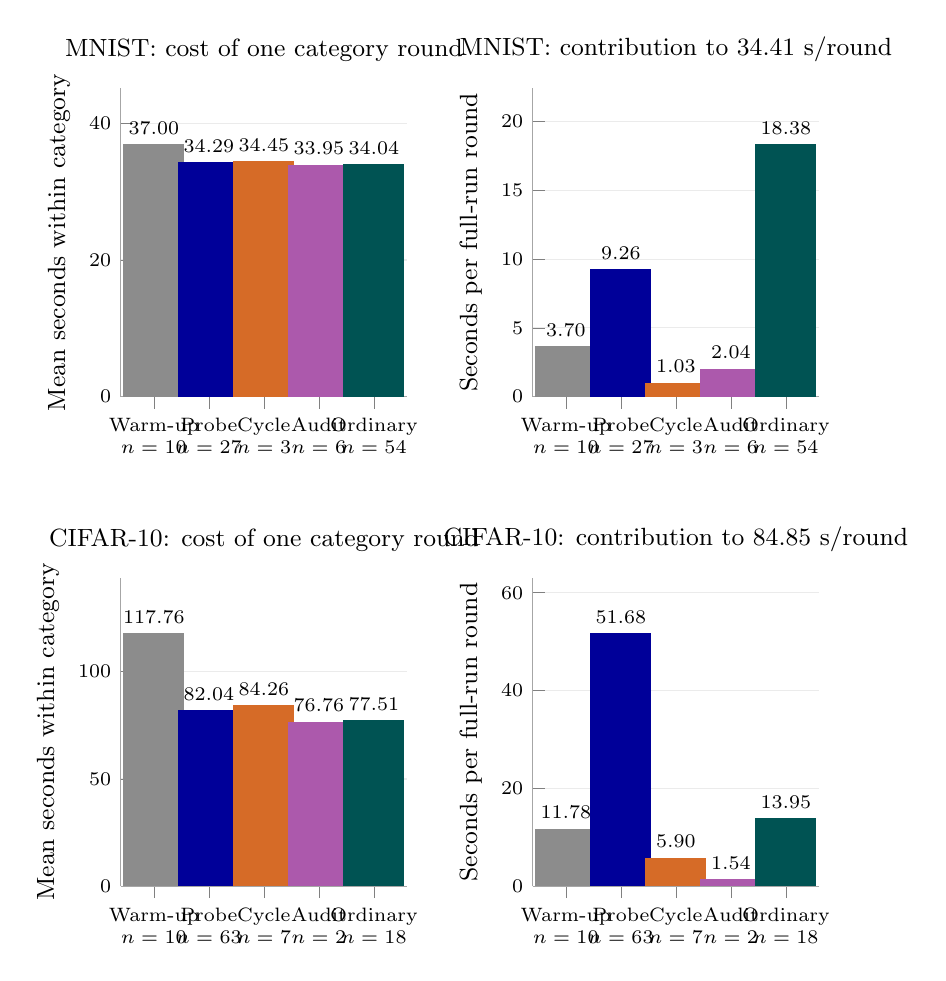
\begin{tikzpicture}
\begin{groupplot}[group style={group size=2 by 2,horizontal sep=1.6cm,vertical sep=2.3cm},
width=0.43\textwidth,height=5.5cm,
grid=major,grid style={black!8},axis line style={black!35},
tick label style={font=\scriptsize},label style={font=\small},title style={font=\small},
legend style={font=\scriptsize,draw=none},scaled y ticks=false]
\nextgroupplot[title={MNIST: cost of one category round},ybar,bar width=22pt,bar shift=0pt,ymin=0,ymax=45.135779,xmin=0.4,xmax=5.6,ylabel={Mean seconds within category},xtick={1,2,3,4,5},xticklabels={{Warm-up\\$n=10$},{Probe\\$n=27$},{Cycle\\$n=3$},{Audit\\$n=6$},{Ordinary\\$n=54$}},xticklabel style={align=center,font=\scriptsize},xmajorgrids=false,axis x line*=bottom,axis y line*=left,nodes near coords,every node near coord/.append style={font=\scriptsize,text=black,/pgf/number format/fixed,/pgf/number format/precision=2,/pgf/number format/fixed zerofill}]
\addplot[fill=black!45,draw=none,bar shift=0pt] coordinates {(1,36.996540260)};
\addplot[fill=blue!60!black,draw=none,bar shift=0pt] coordinates {(2,34.288500330)};
\addplot[fill=riderorange,draw=none,bar shift=0pt] coordinates {(3,34.450482100)};
\addplot[fill=violet!65,draw=none,bar shift=0pt] coordinates {(4,33.951632300)};
\addplot[fill=teal!65!black,draw=none,bar shift=0pt] coordinates {(5,34.036154717)};
\nextgroupplot[title={MNIST: contribution to 34.41 s/round},ybar,bar width=22pt,bar shift=0pt,ymin=0,ymax=22.423019,xmin=0.4,xmax=5.6,ylabel={Seconds per full-run round},xtick={1,2,3,4,5},xticklabels={{Warm-up\\$n=10$},{Probe\\$n=27$},{Cycle\\$n=3$},{Audit\\$n=6$},{Ordinary\\$n=54$}},xticklabel style={align=center,font=\scriptsize},xmajorgrids=false,axis x line*=bottom,axis y line*=left,nodes near coords,every node near coord/.append style={font=\scriptsize,text=black,/pgf/number format/fixed,/pgf/number format/precision=2,/pgf/number format/fixed zerofill}]
\addplot[fill=black!45,draw=none,bar shift=0pt] coordinates {(1,3.699654026)};
\addplot[fill=blue!60!black,draw=none,bar shift=0pt] coordinates {(2,9.257895089)};
\addplot[fill=riderorange,draw=none,bar shift=0pt] coordinates {(3,1.033514463)};
\addplot[fill=violet!65,draw=none,bar shift=0pt] coordinates {(4,2.037097938)};
\addplot[fill=teal!65!black,draw=none,bar shift=0pt] coordinates {(5,18.379523547)};
\nextgroupplot[title={CIFAR-10: cost of one category round},ybar,bar width=22pt,bar shift=0pt,ymin=0,ymax=143.668467,xmin=0.4,xmax=5.6,ylabel={Mean seconds within category},xtick={1,2,3,4,5},xticklabels={{Warm-up\\$n=10$},{Probe\\$n=63$},{Cycle\\$n=7$},{Audit\\$n=2$},{Ordinary\\$n=18$}},xticklabel style={align=center,font=\scriptsize},xmajorgrids=false,axis x line*=bottom,axis y line*=left,nodes near coords,every node near coord/.append style={font=\scriptsize,text=black,/pgf/number format/fixed,/pgf/number format/precision=2,/pgf/number format/fixed zerofill}]
\addplot[fill=black!45,draw=none,bar shift=0pt] coordinates {(1,117.761038190)};
\addplot[fill=blue!60!black,draw=none,bar shift=0pt] coordinates {(2,82.037953983)};
\addplot[fill=riderorange,draw=none,bar shift=0pt] coordinates {(3,84.261838643)};
\addplot[fill=violet!65,draw=none,bar shift=0pt] coordinates {(4,76.756039800)};
\addplot[fill=teal!65!black,draw=none,bar shift=0pt] coordinates {(5,77.510055911)};
\nextgroupplot[title={CIFAR-10: contribution to 84.85 s/round},ybar,bar width=22pt,bar shift=0pt,ymin=0,ymax=63.054371,xmin=0.4,xmax=5.6,ylabel={Seconds per full-run round},xtick={1,2,3,4,5},xticklabels={{Warm-up\\$n=10$},{Probe\\$n=63$},{Cycle\\$n=7$},{Audit\\$n=2$},{Ordinary\\$n=18$}},xticklabel style={align=center,font=\scriptsize},xmajorgrids=false,axis x line*=bottom,axis y line*=left,nodes near coords,every node near coord/.append style={font=\scriptsize,text=black,/pgf/number format/fixed,/pgf/number format/precision=2,/pgf/number format/fixed zerofill}]
\addplot[fill=black!45,draw=none,bar shift=0pt] coordinates {(1,11.776103819)};
\addplot[fill=blue!60!black,draw=none,bar shift=0pt] coordinates {(2,51.683911009)};
\addplot[fill=riderorange,draw=none,bar shift=0pt] coordinates {(3,5.898328705)};
\addplot[fill=violet!65,draw=none,bar shift=0pt] coordinates {(4,1.535120796)};
\addplot[fill=teal!65!black,draw=none,bar shift=0pt] coordinates {(5,13.951810064)};
\end{groupplot}\end{tikzpicture}
\caption{Where our 100-round runtime is spent (non-IID FR3, seed 42, 40\% free riders). Rows separate MNIST and CIFAR-10. Left: mean duration of a complete round in each category. Right: summed duration for that category divided by 100; the five bars add to the full-run mean printed in the title. Labels give category counts $n$. Probe excludes cycle-decision rounds; Cycle includes the final cycle decision; Audit is a single audit round. Categories are mutually exclusive. A cycle bar includes client training, aggregation and evaluation: it is NOT detector-only time. Axes scale independently; all bars start at zero.}\label{fig:timing-phases}
\end{figure*}

\begin{figure*}[tp]\centering\begin{tikzpicture}
\begin{groupplot}[group style={group size=2 by 1,horizontal sep=1.6cm,vertical sep=1.6cm},
width=0.43\textwidth,height=6.4cm,
grid=major,grid style={black!8},axis line style={black!35},
tick label style={font=\scriptsize},label style={font=\small},title style={font=\small},
legend style={font=\scriptsize,draw=none},scaled y ticks=false]
\nextgroupplot[title={MNIST},xmin=0,xmax=101,ymin=0,xlabel={Round},ylabel={Measured seconds},xtick={1,20,40,60,80,100},legend to name=timing-trace-legend,legend columns=3]
\addplot[black!65,thick] table[x=round,y=seconds] {\TimingDataDir/timeline_mnist.dat};
\addlegendentry{Ours: actual 100 rounds}
\addplot[only marks,mark=*,mark size=2pt,color=riderorange] table[x=round,y=seconds] {\TimingDataDir/cycle_rounds_mnist.dat};
\addlegendentry{Full-cycle decision rounds}
\addplot[blue!70!black,thick] table[x=round,y=seconds] {\TimingDataDir/std_rounds_mnist.dat};
\addlegendentry{STD: actual rounds 1--100}
\nextgroupplot[title={CIFAR-10},xmin=0,xmax=101,ymin=0,xlabel={Round},ylabel={Measured seconds},xtick={1,20,40,60,80,100}]
\addplot[black!65,thick] table[x=round,y=seconds] {\TimingDataDir/timeline_cifar10.dat};
\addplot[only marks,mark=*,mark size=2pt,color=riderorange] table[x=round,y=seconds] {\TimingDataDir/cycle_rounds_cifar10.dat};
\addplot[blue!70!black,thick] table[x=round,y=seconds] {\TimingDataDir/std_rounds_cifar10.dat};
\end{groupplot}\end{tikzpicture}
\par\ref{timing-trace-legend}
\caption{Actual per-round durations over 100 executed rounds for both methods. Our trajectories include changing active-client counts and probing schedules; STD-DAGMM retains all 100 clients. Markers indicate full-cycle decisions, not their isolated computational cost. Axis scales differ by dataset.}\label{fig:timing-traces}
\end{figure*}



\FloatBarrier
\section{Result Analysis}
\subsection{Effect of Attack Behavior}
\textbf{FR1} is consistently removed at the earliest allowed round. Exact
sendback provides a distinct evidence path, so its success does not validate
the statistical separation gate. Near-converged honest zero updates would
still require separate examination in other training regimes.

\textbf{FR2} is removed by round 30 in all settings despite avoiding equality.
The observed responses are sufficiently distinct under the configured random
update distribution and repeated traps. This is evidence about the tested
amplitude, not proof that arbitrary fabricated noise will be detected.

\textbf{FR3} is the critical heterogeneous-data case. Its current-inclusive
history can yield responses that overlap honest update geometry. In non-IID
CIFAR-10 at 40\%, all 40 free riders receive full norm certificates at rounds
20 and 60; at 30\%, all 30 receive them at rounds 40 and 80. Ambiguous intervening
cycles do not increment these counts. Retention permits the later fresh
certificate to confirm removal. This recorded sequence explains how the memory
rule operates; it is not a matched ablation proving that memory alone caused
the outcome under a counterfactual training trajectory.

\textbf{FR4} is removed by round 30 in the present grid. Its received-trajectory
estimate includes traps, which plausibly contributes to separation from genuine
optimization. This is an interpretation of the mechanism, not a measurement of
the attacker's inference ability. A defense-aware attacker could treat repeated
or unusual received states differently and needs a separate evaluation.

\subsection{Dataset, Partition, and Attacker Share}
MNIST completes removal early in every condition, while non-IID CIFAR-10 FR3
requires additional evidence cycles. This shows that neither attack identity
alone nor final recall fully describes difficulty. The interaction between
honest-data heterogeneity, model state, and fabricated response geometry matters.

Changing the share from 40\% to 30\% preserves complete detection but delays
the difficult CIFAR-10 FR3 case from round 60 to round 80. A lower attacker
share therefore does not imply faster discovery. Cohort support and the
distribution of the surrounding honest population both change; the server does
not use the known simulation share to force a quota or boundary.

The 30\% runs also train 70 honest clients rather than 60. This increases
genuine local work and helps explain longer simulator round times without
implying a more expensive statistical rule. Non-IID client dataset sizes differ,
so the increase need not equal the 16.7\% change in honest-client count.
The slightly higher achieved accuracies at 30\% are consistent with more honest
training, but no causal effect is established without matched controls.

\subsection{Screening Quality Versus Removal Safety}
The central positive result is that repeated-evidence gating prevents permanent
honest removal in these 100-round trajectories, even when screening is noisy.
The central unresolved issue is that some non-IID honest populations remain
almost entirely candidate-labelled after attackers disappear. This can arise
when relative statistical comparisons continue to find weak differences among
honest clients. Such labels do not, by themselves, exclude ordinary updates,
but they limit the meaning of calling R ``safe'' or C ``malicious.'' We interpret
R as unflagged, C as unresolved, and S as freshly certified suspicion.

Temporary exclusion also remains a real cost. Most honest exclusions are
deliberate trap responses, not quarantine. In ordinary successful MNIST runs,
660 honest client-rounds are withheld at 40\% and 770 at 30\%, corresponding
to eleven trap rounds per honest client over the 100-round horizon. The
exceptional FR3 follow-up adds further probing. A deployment should measure
whether this forgone aggregation delays reaching a target utility, rather
than reporting permanent-removal precision alone.

\subsection{What the Current Evidence Does Not Establish}
The current grid has no held-out seed, honest-only control, long-horizon test,
matched ablation, or baseline comparison under identical trajectories. We cannot
estimate cross-seed variability, claim statistical independence of all client-cases,
or infer universal 100\% recall. Variations of attacker history length, noise
amplitude, trap strength, local epoch count, non-IID concentration, and model
architecture remain necessary robustness tests. In particular, the influence of
CIFAR BatchNorm buffers should be separated from trainable-weight evidence.

\section{Complexity and Lightweight Design}\label{sec:complexity}
\subsection{Operation Counts and Scaling}
Let $N$ be active clients, $P$ floating model coordinates (including floating
buffers), $L$ floating tensors, $T$ rounds, $B$ bootstrap replicates and
$K=\lceil\sqrt{N}\rceil$ histogram bins. The following are implementation
bounds, not measured wall-clock predictions. We count model scanning separately
from local optimization and ordinary aggregation.

\begin{table*}[t]\centering\footnotesize
\caption{Incremental detector operations and working state. ``Cycle'' means a complete A/B evidence cycle; it does not mean every training round. Bounds exclude ordinary model aggregation, local training, simulator attack histories and persistent logging.}\label{tab:complexity}
\begin{tabular}{p{3.6cm}p{3.6cm}p{3.0cm}p{5.3cm}}\toprule
Component & Work & Working state & Practical interpretation \\ \midrule
Norm, profile, exact fingerprint & $O(NP)$ per round & $O(P)$ scratch, $O(N)$ fingerprints & Sequential model reads; no auxiliary training or gradients. \\
Selected A/B summaries & $O(NL)$ per cycle to store & $O(NL)$ & Two compact profiles per active client, not full response histories. \\
Leave-one-out norm/profile scores & $O(N^2(L+\log N))$ per cycle & $O(NL)$ temporary & Repeated peer-profile medians/distances; Python scalar medians sort. \\
Three histogram/bootstrap views & $O(B(N+K))$ per cycle & $O(BN+BK)$ scratch & Three views add a constant factor; $B=1000$. \\
Geometric gates and memory & $O(N)$ selections/quantiles per cycle & $O(N)$ counters & Fixed component count; no learned detector or history-window reconstruction. \\
Two model challenges & $O(P)$ generation per cycle & $O(P)$ & Two shared trap states, not a distinct trap model per client. \\
\bottomrule\end{tabular}\end{table*}

The leave-one-out implementation rebuilds $N-1$ peer profiles for every
client and trap. Profile medians and distances require $O(N^2L)$ coordinate
work; repeated scalar medians in Python's \texttt{statistics.median} add
$O(N^2\log N)$ sorting work. Thus, calling the whole method linear in client
count would be incorrect. Histogram binning and bootstrap resampling operate
only on scalar scores, not on $P$-dimensional model vectors. With $M$ complete
cycles, the detector work is bounded by
\begin{equation}
\begin{aligned}
 W={}&O\bigl(TNP\bigr)\\
 &+O\!\left(M\left[N^2(L+\log N)+B(N+K)\right]\right).
\end{aligned}
\end{equation}
Single-trap audits add corresponding one-view scoring passes; they cannot
authorize permanent removal. Dense monitoring supplies more observations but
only one preselected A/B pair per client enters each complete-cycle decision.

At $N=100$, the two-trap profile comparison visits
$2N(N-1)L=158{,}400$ profile coordinates for MNIST and $435{,}600$ for CIFAR-10,
before constants for medians and distances. One bootstrap view draws $BN=100{,}000$
scalar indices; three views process three such sets using reused draws in the
current implementation. These counts explain why the evidence layer is compact
relative to repeated full-model training, but they do not measure its elapsed time.

\subsection{Payload Sizes, Memory Boundaries and Communication}
Table~\ref{tab:payload} derives concrete payload sizes from the implemented
architectures. The compact float32 pair payload is
$2N(L+3)\cdot4$ bytes under the stated packed representation; the three scalar
slots are an illustrative norm/round/flag allowance, not the actual Python object
layout. The two trap models occupy $2P\cdot4$ floating bytes. Actual dictionaries,
lists, Python scalars, allocator overhead, fingerprints and bootstrap temporaries
increase memory. For example, bootstrap index gathers and bin-index arrays coexist
with resample/count arrays; their two listed sizes must not be relabelled as peak
bootstrap RSS.
\begin{table*}[t]\centering\footnotesize
\caption{Calculated detector payload sizes at $N=100$, two traps, $B=1000$: architecture-derived estimates, NOT measured heap usage.}\label{tab:payload}
\begin{tabular}{lrrrrrrr}\toprule
Model & Parameters & $P$ & $L$ & Two traps (MiB) & Pair payload (KiB) & Index array (MiB) & Counts (MiB) \\ \midrule
MNIST & 206922 & 206922 & 8 & 1.579 & 8.594 & 0.763 & 0.076 \\
CIFAR-10 & 620810 & 621258 & 22 & 4.740 & 19.531 & 0.763 & 0.076 \\
\bottomrule\end{tabular}
\par\smallskip\begin{minipage}{0.96\textwidth}\scriptsize $P$ includes floating BatchNorm buffers; $L$ counts floating tensors. Pair payload assumes packed float32 profiles plus three scalar slots per trap/client. Bootstrap columns show two principal arrays, not peak scratch or an upper bound. No detector-only RSS was recorded.\end{minipage}\end{table*}


The decision working state is $O(P+NL+BN+BK)$, plus $O(N)$ counters and
fingerprints. In contrast, the research logger accumulates per-round/probe rows,
including tensor profiles, so the full simulator's retained evidence can grow
as $O(TNL)$ in dense probing. Ordinary aggregation also retains model responses,
and the simulator stores attack histories. The measured process RSS in
Table~\ref{tab:cost} includes these costs; it is not evidence that the entire
implementation uses only compact decision-state memory. Streaming logs and
aggregation would be deployment optimizations, not features benchmarked here.

No extra local optimization pass or auxiliary classifier is required. Under the
existing full-participation request/response schedule, traps replace ordinary
models rather than adding a second exchange; challenge responses are discarded
from aggregation. The nominal model-payload order remains $O(NP)$ per round,
excluding transport/serialization overhead. This does not make communication
``free'': useful contributions are withheld, so reaching a target accuracy can
require more rounds. Network-byte measurements and controlled detector-only
profiling are still necessary. We use \emph{lightweight} to mean compact features,
no auxiliary learning, and constant-sized per-client evidence memory, not an
unmeasured universal speed or energy advantage.

\section{Security Analysis}
\subsection{Decision Inputs and Attack-Label Separation}
The detector receives an allowlist of client/trap IDs, raw norms, profile
distances, robust scores, and exact-sendback indicators. The simulator's attacker
labels and behavior choices are not passed to screening, geometric tests, or
the client state machine. Evaluation prevalence determines how many attackers
the simulator creates, not how many removals the detector attempts to achieve.
This code boundary reduces direct evaluation leakage; it does not make the
development process independent of previously observed results.

\subsection{Confirmation Invariants}
Three operational safeguards follow from the state-transition rules.
First, statistical removal requires the same component on both selected traps
and a second distinct full cycle: one trap, mixed norm/profile evidence, or
an ambiguous result cannot independently supply the required confirmation.
Second, previously stored evidence does not authorize a new removal without
a fresh current certificate. Third, stored counts and weak C evidence cannot
renew quarantine; unconfirmed review expires unless fresh strong evidence
returns. These are protocol invariants, not probabilistic security bounds.

The guarantees are intentionally narrower than ``no false positives.'' An
honest client can satisfy the same geometric gate in two cycles. A clean
majority and independent trap draws do not make the resulting statistical
certificates independent, because clients retain the same data and related
model trajectories.

\subsection{Evasion, Identifiability, and Trap Secrecy}
Consider two executions with identical server-observable response histories,
public identities, and server randomness, one produced by honest training and
the other by fabrication. A detector whose transition function depends only on
those observations has the same state trajectory in both executions. Therefore,
update-only screening cannot prove genuine computation against every attacker.
The proposed method must be evaluated by how well its challenges separate
specified behaviors, not as a cryptographic proof of training.

The evaluated attackers are not given trap labels, but several real-world
signals could reveal auditing: repeated frozen states, abrupt distributional
changes, or communication between clients receiving different models. Moreover,
the simulator derives reproducible randomness from configured seeds; it does
not establish unpredictability against an adversary that knows those seeds.
Deployment would require server-secret randomness and an evaluation of
defense-aware response strategies. Even secret randomness alone would not
establish indistinguishability of traps from ordinary models.

\subsection{Honest-Client Safety and Long-Term Accumulation}
There is no fitted numerical z-score cutoff for statistical removal, but the
policy is not parameter-free. Trap scale, histogram binning, bootstrap confidence,
cohort support, confirmation count, and review/clearance lengths are design
choices. A stable boundary is not a calibrated false-removal probability.
At 100 clients the minimum statistical cohort support is ten; an isolated
nonzero free rider can therefore escape this cohort gate.

Certificate memory deliberately has no fixed age limit. If an honest client's
atypical geometry generates repeated strong evidence without two complete R
cycles, it can eventually be removed. The profile gate's concentration
alternative and persistent candidate populations make this a material
long-horizon risk. The absence of honest removals through round 100 cannot
exclude it. Longer honest-only and heterogeneous-population experiments are
needed before making deployment safety claims.

\subsection{Privacy, Collusion, and Availability}
The protocol is not directly compatible with standard secure aggregation and
does not provide differential privacy~\cite{bonawitz2017practical}. Avoiding
client-reported loss and raw data access reduces required inputs but is not a
privacy proof: identifiable returned models may still leak information.
Colluding clients could share a genuinely trained response or infer the trap
schedule, and Sybil identities could distort the assumed honest-majority
reference. Neither attack is evaluated.

All active clients and complete A/B coverage are required for a certifying
cycle. Missing/nonfinite measurements cannot certify, and the current simulator
aborts on a nonfinite client response rather than implementing a complete
availability defense. Dropout tolerance, malicious-message handling, restart
integrity, authentication, and denial-of-service resistance require additional
engineering and experiments. Checkpoint recovery preserves computation and
evidence state after interruption; it does not create new evidence of honesty.

\subsection{Computational and Communication Exposure}
The bounds in Section~\ref{sec:complexity} expose quadratic-in-population
leave-one-out work and transient bootstrap memory. A large population or model
can make auditing expensive even without learned detector training. Deliberately
withheld trap responses and repeated honest follow-up are an availability and
utility cost, not merely an implementation detail. Communication bytes, time to
target utility, energy, and isolated detector work remain unmeasured.

\section{Conclusion}
This study evaluates a lightweight, server-observable challenge approach to
free-rider screening, with strict norm separation, component-specific evidence
memory, and bounded review. Across 32 completed MNIST/CIFAR-10 runs, all 1,120
free-rider client-cases are removed with no permanent honest removal. Most
conditions complete by round 30; non-IID CIFAR-10 history averaging requires
rounds 60 and 80. The result shows useful separation under the evaluated
training and attack configurations, while the candidate and quarantine results
show why final recall and precision alone are insufficient.

The principal next step is validation, not further adjustment to this seed:
freeze the policy, evaluate unseen seeds and honest-only populations, and test
adaptive/mixed attacks and longer horizons. Matched ablations and detector-only
profiling should distinguish the contributions of traps, geometric gates, and
memory from ordinary training and simulator costs. The method is a promising
empirical screening mechanism, not a universal verifier of local computation.

\FloatBarrier
\appendices
\section{Complete Per-Run Results}
Tables~\ref{tab:detail-mnist} and~\ref{tab:detail-cifar10} retain every evaluated
attack/partition/share combination. Machine-readable exports include per-run
statistics, grouped summaries, full-cycle certificate histories, and per-round
curves. No failed run is omitted or converted into a blank value.
\begin{table*}[t]
\centering\footnotesize\setlength{\tabcolsep}{4pt}
\caption{Complete per-run MNIST outcomes. Every run has 100 rounds and seed 42. Definitions match Tables~\ref{tab:performance} and~\ref{tab:safety}; all outcomes, including failures if present, are retained.}\label{tab:detail-mnist}
\begin{tabular}{rllrrrrrrrr}
\toprule
FR (\%) & Partition & Attack & TP & FP & FN & $t_{\rm all}$ & Accuracy (\%) & $C_H$ & $Q_H$ & $q_H$ \\
\midrule
30 & IID & FR1 & 30 & 0 & 0 & 30 & 99.02 & 1 & 0 & 0 \\
30 & IID & FR2 & 30 & 0 & 0 & 30 & 99.00 & 5 & 0 & 0 \\
30 & IID & FR3 & 30 & 0 & 0 & 30 & 99.00 & 8 & 0 & 0 \\
30 & IID & FR4 & 30 & 0 & 0 & 30 & 98.82 & 2 & 0 & 0 \\
30 & Non-IID & FR1 & 30 & 0 & 0 & 30 & 99.01 & 7 & 0 & 0 \\
30 & Non-IID & FR2 & 30 & 0 & 0 & 30 & 99.00 & 6 & 0 & 0 \\
30 & Non-IID & FR3 & 30 & 0 & 0 & 30 & 98.98 & 8 & 0 & 0 \\
30 & Non-IID & FR4 & 30 & 0 & 0 & 30 & 98.96 & 6 & 0 & 0 \\
40 & IID & FR1 & 40 & 0 & 0 & 30 & 98.90 & 1 & 0 & 0 \\
40 & IID & FR2 & 40 & 0 & 0 & 30 & 98.91 & 5 & 0 & 0 \\
40 & IID & FR3 & 40 & 0 & 0 & 30 & 98.85 & 5 & 0 & 0 \\
40 & IID & FR4 & 40 & 0 & 0 & 30 & 98.77 & 5 & 0 & 0 \\
40 & Non-IID & FR1 & 40 & 0 & 0 & 30 & 98.96 & 2 & 0 & 0 \\
40 & Non-IID & FR2 & 40 & 0 & 0 & 30 & 98.96 & 7 & 0 & 0 \\
40 & Non-IID & FR3 & 40 & 0 & 0 & 30 & 98.93 & 34 & 1 & 20 \\
40 & Non-IID & FR4 & 40 & 0 & 0 & 30 & 98.98 & 12 & 0 & 0 \\
\bottomrule
\end{tabular}

\end{table*}

\begin{table*}[t]
\centering\footnotesize\setlength{\tabcolsep}{4pt}
\caption{Complete per-run CIFAR-10 outcomes. Every run has 100 rounds and seed 42. Definitions match Tables~\ref{tab:performance} and~\ref{tab:safety}; all outcomes, including failures if present, are retained.}\label{tab:detail-cifar10}
\begin{tabular}{rllrrrrrrrr}
\toprule
FR (\%) & Partition & Attack & TP & FP & FN & $t_{\rm all}$ & Accuracy (\%) & $C_H$ & $Q_H$ & $q_H$ \\
\midrule
30 & IID & FR1 & 30 & 0 & 0 & 30 & 78.07 & 2 & 0 & 0 \\
30 & IID & FR2 & 30 & 0 & 0 & 30 & 77.93 & 0 & 0 & 0 \\
30 & IID & FR3 & 30 & 0 & 0 & 30 & 78.17 & 2 & 0 & 0 \\
30 & IID & FR4 & 30 & 0 & 0 & 30 & 78.03 & 7 & 0 & 0 \\
30 & Non-IID & FR1 & 30 & 0 & 0 & 30 & 75.80 & 8 & 0 & 0 \\
30 & Non-IID & FR2 & 30 & 0 & 0 & 30 & 75.58 & 2 & 0 & 0 \\
30 & Non-IID & FR3 & 30 & 0 & 0 & 80 & 75.36 & 70 & 1 & 20 \\
30 & Non-IID & FR4 & 30 & 0 & 0 & 30 & 75.78 & 7 & 0 & 0 \\
40 & IID & FR1 & 40 & 0 & 0 & 30 & 77.46 & 0 & 0 & 0 \\
40 & IID & FR2 & 40 & 0 & 0 & 30 & 77.65 & 0 & 0 & 0 \\
40 & IID & FR3 & 40 & 0 & 0 & 30 & 77.27 & 4 & 0 & 0 \\
40 & IID & FR4 & 40 & 0 & 0 & 30 & 77.36 & 8 & 0 & 0 \\
40 & Non-IID & FR1 & 40 & 0 & 0 & 30 & 75.28 & 9 & 0 & 0 \\
40 & Non-IID & FR2 & 40 & 0 & 0 & 30 & 75.43 & 4 & 0 & 0 \\
40 & Non-IID & FR3 & 40 & 0 & 0 & 60 & 74.89 & 52 & 9 & 180 \\
40 & Non-IID & FR4 & 40 & 0 & 0 & 30 & 75.14 & 7 & 0 & 0 \\
\bottomrule
\end{tabular}

\end{table*}


\section{Supporting Trajectories and Score Geometry}\label{app:trajectories}
Figure~\ref{fig:recall} retains all cumulative detection trajectories, including
the delayed non-IID CIFAR-10 FR3 cases. Figure~\ref{fig:accuracy-overview} restores
the full training horizon and shared 0--1 scale for interpreting the main-text
accuracy zooms. Figures~\ref{fig:scatter-mnist-30} and
\ref{fig:scatter-cifar10-30} show the complementary 30\% client clouds using
the same paired-score definition and monotone display transformation.
\begin{figure*}[tp]\centering
\begin{tikzpicture}
\begin{groupplot}[group style={group size=2 by 4,horizontal sep=0.9cm,vertical sep=1.25cm},
width=0.455\textwidth,height=4.6cm,xmin=0,xmax=100,
ymin=0,ymax=1.05,
grid=major,xtick={0,30,60,100},tick label style={font=\scriptsize},
title style={font=\small},label style={font=\scriptsize},legend style={font=\scriptsize,draw=none},
legend columns=4]
\nextgroupplot[title={MNIST FR1},ylabel={Removal recall},legend to name=fig:recall-legend]
\addplot[blue,solid,thick,const plot] table[x=round,y=recall] {generated/mnist_iid_FR1_p30.dat};
\addlegendentry{30\% IID}
\addplot[red!80!black,dashed,thick,const plot] table[x=round,y=recall] {generated/mnist_noniid_FR1_p30.dat};
\addlegendentry{30\% Non-IID}
\addplot[teal!70!black,dotted,thick,const plot] table[x=round,y=recall] {generated/mnist_iid_FR1_p40.dat};
\addlegendentry{40\% IID}
\addplot[orange!90!black,dashdotted,thick,const plot] table[x=round,y=recall] {generated/mnist_noniid_FR1_p40.dat};
\addlegendentry{40\% Non-IID}
\nextgroupplot[title={MNIST FR2}]
\addplot[blue,solid,thick,const plot] table[x=round,y=recall] {generated/mnist_iid_FR2_p30.dat};
\addplot[red!80!black,dashed,thick,const plot] table[x=round,y=recall] {generated/mnist_noniid_FR2_p30.dat};
\addplot[teal!70!black,dotted,thick,const plot] table[x=round,y=recall] {generated/mnist_iid_FR2_p40.dat};
\addplot[orange!90!black,dashdotted,thick,const plot] table[x=round,y=recall] {generated/mnist_noniid_FR2_p40.dat};
\nextgroupplot[title={MNIST FR3}]
\addplot[blue,solid,thick,const plot] table[x=round,y=recall] {generated/mnist_iid_FR3_p30.dat};
\addplot[red!80!black,dashed,thick,const plot] table[x=round,y=recall] {generated/mnist_noniid_FR3_p30.dat};
\addplot[teal!70!black,dotted,thick,const plot] table[x=round,y=recall] {generated/mnist_iid_FR3_p40.dat};
\addplot[orange!90!black,dashdotted,thick,const plot] table[x=round,y=recall] {generated/mnist_noniid_FR3_p40.dat};
\nextgroupplot[title={MNIST FR4}]
\addplot[blue,solid,thick,const plot] table[x=round,y=recall] {generated/mnist_iid_FR4_p30.dat};
\addplot[red!80!black,dashed,thick,const plot] table[x=round,y=recall] {generated/mnist_noniid_FR4_p30.dat};
\addplot[teal!70!black,dotted,thick,const plot] table[x=round,y=recall] {generated/mnist_iid_FR4_p40.dat};
\addplot[orange!90!black,dashdotted,thick,const plot] table[x=round,y=recall] {generated/mnist_noniid_FR4_p40.dat};
\nextgroupplot[title={CIFAR-10 FR1},ylabel={Removal recall}]
\addplot[blue,solid,thick,const plot] table[x=round,y=recall] {generated/cifar10_iid_FR1_p30.dat};
\addplot[red!80!black,dashed,thick,const plot] table[x=round,y=recall] {generated/cifar10_noniid_FR1_p30.dat};
\addplot[teal!70!black,dotted,thick,const plot] table[x=round,y=recall] {generated/cifar10_iid_FR1_p40.dat};
\addplot[orange!90!black,dashdotted,thick,const plot] table[x=round,y=recall] {generated/cifar10_noniid_FR1_p40.dat};
\nextgroupplot[title={CIFAR-10 FR2}]
\addplot[blue,solid,thick,const plot] table[x=round,y=recall] {generated/cifar10_iid_FR2_p30.dat};
\addplot[red!80!black,dashed,thick,const plot] table[x=round,y=recall] {generated/cifar10_noniid_FR2_p30.dat};
\addplot[teal!70!black,dotted,thick,const plot] table[x=round,y=recall] {generated/cifar10_iid_FR2_p40.dat};
\addplot[orange!90!black,dashdotted,thick,const plot] table[x=round,y=recall] {generated/cifar10_noniid_FR2_p40.dat};
\nextgroupplot[title={CIFAR-10 FR3},xlabel={Round}]
\addplot[blue,solid,thick,const plot] table[x=round,y=recall] {generated/cifar10_iid_FR3_p30.dat};
\addplot[red!80!black,dashed,thick,const plot] table[x=round,y=recall] {generated/cifar10_noniid_FR3_p30.dat};
\addplot[teal!70!black,dotted,thick,const plot] table[x=round,y=recall] {generated/cifar10_iid_FR3_p40.dat};
\addplot[orange!90!black,dashdotted,thick,const plot] table[x=round,y=recall] {generated/cifar10_noniid_FR3_p40.dat};
\nextgroupplot[title={CIFAR-10 FR4},xlabel={Round}]
\addplot[blue,solid,thick,const plot] table[x=round,y=recall] {generated/cifar10_iid_FR4_p30.dat};
\addplot[red!80!black,dashed,thick,const plot] table[x=round,y=recall] {generated/cifar10_noniid_FR4_p30.dat};
\addplot[teal!70!black,dotted,thick,const plot] table[x=round,y=recall] {generated/cifar10_iid_FR4_p40.dat};
\addplot[orange!90!black,dashdotted,thick,const plot] table[x=round,y=recall] {generated/cifar10_noniid_FR4_p40.dat};
\end{groupplot}\end{tikzpicture}
\par\ref{fig:recall-legend}
\caption{Cumulative free-rider removal recall in all 32 runs. Enlarged two-column panels identify dataset and attack in each title; the four lines distinguish partition and attacker share. Coincident curves overlap. Complete outcomes are retained, including incomplete detection if present.}\label{fig:recall}
\end{figure*}

\begin{figure*}[tp]\centering
\begin{tikzpicture}
\begin{groupplot}[group style={group size=2 by 4,horizontal sep=0.9cm,vertical sep=1.25cm},
width=0.455\textwidth,height=4.6cm,xmin=0,xmax=100,
ymin=0,ymax=1.02,
grid=major,xtick={0,30,60,100},tick label style={font=\scriptsize},
title style={font=\small},label style={font=\scriptsize},legend style={font=\scriptsize,draw=none},
legend columns=4]
\nextgroupplot[title={MNIST FR1},ylabel={Test accuracy},legend to name=fig:accuracy-overview-legend]
\addplot[blue,solid,thick] table[x=round,y=accuracy] {generated/mnist_iid_FR1_p30.dat};
\addlegendentry{30\% IID}
\addplot[red!80!black,dashed,thick] table[x=round,y=accuracy] {generated/mnist_noniid_FR1_p30.dat};
\addlegendentry{30\% Non-IID}
\addplot[teal!70!black,dotted,thick] table[x=round,y=accuracy] {generated/mnist_iid_FR1_p40.dat};
\addlegendentry{40\% IID}
\addplot[orange!90!black,dashdotted,thick] table[x=round,y=accuracy] {generated/mnist_noniid_FR1_p40.dat};
\addlegendentry{40\% Non-IID}
\nextgroupplot[title={MNIST FR2}]
\addplot[blue,solid,thick] table[x=round,y=accuracy] {generated/mnist_iid_FR2_p30.dat};
\addplot[red!80!black,dashed,thick] table[x=round,y=accuracy] {generated/mnist_noniid_FR2_p30.dat};
\addplot[teal!70!black,dotted,thick] table[x=round,y=accuracy] {generated/mnist_iid_FR2_p40.dat};
\addplot[orange!90!black,dashdotted,thick] table[x=round,y=accuracy] {generated/mnist_noniid_FR2_p40.dat};
\nextgroupplot[title={MNIST FR3}]
\addplot[blue,solid,thick] table[x=round,y=accuracy] {generated/mnist_iid_FR3_p30.dat};
\addplot[red!80!black,dashed,thick] table[x=round,y=accuracy] {generated/mnist_noniid_FR3_p30.dat};
\addplot[teal!70!black,dotted,thick] table[x=round,y=accuracy] {generated/mnist_iid_FR3_p40.dat};
\addplot[orange!90!black,dashdotted,thick] table[x=round,y=accuracy] {generated/mnist_noniid_FR3_p40.dat};
\nextgroupplot[title={MNIST FR4}]
\addplot[blue,solid,thick] table[x=round,y=accuracy] {generated/mnist_iid_FR4_p30.dat};
\addplot[red!80!black,dashed,thick] table[x=round,y=accuracy] {generated/mnist_noniid_FR4_p30.dat};
\addplot[teal!70!black,dotted,thick] table[x=round,y=accuracy] {generated/mnist_iid_FR4_p40.dat};
\addplot[orange!90!black,dashdotted,thick] table[x=round,y=accuracy] {generated/mnist_noniid_FR4_p40.dat};
\nextgroupplot[title={CIFAR-10 FR1},ylabel={Test accuracy}]
\addplot[blue,solid,thick] table[x=round,y=accuracy] {generated/cifar10_iid_FR1_p30.dat};
\addplot[red!80!black,dashed,thick] table[x=round,y=accuracy] {generated/cifar10_noniid_FR1_p30.dat};
\addplot[teal!70!black,dotted,thick] table[x=round,y=accuracy] {generated/cifar10_iid_FR1_p40.dat};
\addplot[orange!90!black,dashdotted,thick] table[x=round,y=accuracy] {generated/cifar10_noniid_FR1_p40.dat};
\nextgroupplot[title={CIFAR-10 FR2}]
\addplot[blue,solid,thick] table[x=round,y=accuracy] {generated/cifar10_iid_FR2_p30.dat};
\addplot[red!80!black,dashed,thick] table[x=round,y=accuracy] {generated/cifar10_noniid_FR2_p30.dat};
\addplot[teal!70!black,dotted,thick] table[x=round,y=accuracy] {generated/cifar10_iid_FR2_p40.dat};
\addplot[orange!90!black,dashdotted,thick] table[x=round,y=accuracy] {generated/cifar10_noniid_FR2_p40.dat};
\nextgroupplot[title={CIFAR-10 FR3},xlabel={Round}]
\addplot[blue,solid,thick] table[x=round,y=accuracy] {generated/cifar10_iid_FR3_p30.dat};
\addplot[red!80!black,dashed,thick] table[x=round,y=accuracy] {generated/cifar10_noniid_FR3_p30.dat};
\addplot[teal!70!black,dotted,thick] table[x=round,y=accuracy] {generated/cifar10_iid_FR3_p40.dat};
\addplot[orange!90!black,dashdotted,thick] table[x=round,y=accuracy] {generated/cifar10_noniid_FR3_p40.dat};
\nextgroupplot[title={CIFAR-10 FR4},xlabel={Round}]
\addplot[blue,solid,thick] table[x=round,y=accuracy] {generated/cifar10_iid_FR4_p30.dat};
\addplot[red!80!black,dashed,thick] table[x=round,y=accuracy] {generated/cifar10_noniid_FR4_p30.dat};
\addplot[teal!70!black,dotted,thick] table[x=round,y=accuracy] {generated/cifar10_iid_FR4_p40.dat};
\addplot[orange!90!black,dashdotted,thick] table[x=round,y=accuracy] {generated/cifar10_noniid_FR4_p40.dat};
\end{groupplot}\end{tikzpicture}
\par\ref{fig:accuracy-overview-legend}
\caption{Full, unzoomed global test-accuracy trajectories for all 32 runs, providing context for the late-training detail in the main text.}\label{fig:accuracy-overview}
\end{figure*}

\begin{figure*}[tp]\centering
\begin{tikzpicture}
\begin{groupplot}[group style={group size=2 by 4,horizontal sep=0.8cm,vertical sep=1.25cm},
width=0.455\textwidth,height=4.6cm,
axis line style={black!35},grid=major,grid style={black!8},
tick label style={font=\scriptsize},title style={font=\small},
label style={font=\scriptsize},legend style={font=\scriptsize,draw=none},
scaled ticks=false,unbounded coords=jump]
\nextgroupplot[title={IID FR1},ylabel={$\operatorname{asinh}(\bar z_{\rm profile})$},legend to name=scatter-mnist-30-legend,legend columns=2]
\addplot[only marks,mark=o,mark size=1.65pt,color=honestblue,opacity=0.7] table[x=x,y=y] {generated/visuals/scatter_mnist_30_iid_FR1_0.dat};
\addlegendentry{Honest}
\addplot[only marks,mark=triangle*,mark size=1.65pt,color=riderorange,opacity=0.7] table[x=x,y=y] {generated/visuals/scatter_mnist_30_iid_FR1_1.dat};
\addlegendentry{Free rider}
\nextgroupplot[title={IID FR2},]
\addplot[only marks,mark=o,mark size=1.65pt,color=honestblue,opacity=0.7] table[x=x,y=y] {generated/visuals/scatter_mnist_30_iid_FR2_0.dat};
\addplot[only marks,mark=triangle*,mark size=1.65pt,color=riderorange,opacity=0.7] table[x=x,y=y] {generated/visuals/scatter_mnist_30_iid_FR2_1.dat};
\nextgroupplot[title={IID FR3},ylabel={$\operatorname{asinh}(\bar z_{\rm profile})$}]
\addplot[only marks,mark=o,mark size=1.65pt,color=honestblue,opacity=0.7] table[x=x,y=y] {generated/visuals/scatter_mnist_30_iid_FR3_0.dat};
\addplot[only marks,mark=triangle*,mark size=1.65pt,color=riderorange,opacity=0.7] table[x=x,y=y] {generated/visuals/scatter_mnist_30_iid_FR3_1.dat};
\nextgroupplot[title={IID FR4},]
\addplot[only marks,mark=o,mark size=1.65pt,color=honestblue,opacity=0.7] table[x=x,y=y] {generated/visuals/scatter_mnist_30_iid_FR4_0.dat};
\addplot[only marks,mark=triangle*,mark size=1.65pt,color=riderorange,opacity=0.7] table[x=x,y=y] {generated/visuals/scatter_mnist_30_iid_FR4_1.dat};
\nextgroupplot[title={Non-IID FR1},ylabel={$\operatorname{asinh}(\bar z_{\rm profile})$}]
\addplot[only marks,mark=o,mark size=1.65pt,color=honestblue,opacity=0.7] table[x=x,y=y] {generated/visuals/scatter_mnist_30_noniid_FR1_0.dat};
\addplot[only marks,mark=triangle*,mark size=1.65pt,color=riderorange,opacity=0.7] table[x=x,y=y] {generated/visuals/scatter_mnist_30_noniid_FR1_1.dat};
\nextgroupplot[title={Non-IID FR2},]
\addplot[only marks,mark=o,mark size=1.65pt,color=honestblue,opacity=0.7] table[x=x,y=y] {generated/visuals/scatter_mnist_30_noniid_FR2_0.dat};
\addplot[only marks,mark=triangle*,mark size=1.65pt,color=riderorange,opacity=0.7] table[x=x,y=y] {generated/visuals/scatter_mnist_30_noniid_FR2_1.dat};
\nextgroupplot[title={Non-IID FR3},xlabel={$\operatorname{asinh}(\bar z_{\rm norm})$},ylabel={$\operatorname{asinh}(\bar z_{\rm profile})$}]
\addplot[only marks,mark=o,mark size=1.65pt,color=honestblue,opacity=0.7] table[x=x,y=y] {generated/visuals/scatter_mnist_30_noniid_FR3_0.dat};
\addplot[only marks,mark=triangle*,mark size=1.65pt,color=riderorange,opacity=0.7] table[x=x,y=y] {generated/visuals/scatter_mnist_30_noniid_FR3_1.dat};
\nextgroupplot[title={Non-IID FR4},xlabel={$\operatorname{asinh}(\bar z_{\rm norm})$}]
\addplot[only marks,mark=o,mark size=1.65pt,color=honestblue,opacity=0.7] table[x=x,y=y] {generated/visuals/scatter_mnist_30_noniid_FR4_0.dat};
\addplot[only marks,mark=triangle*,mark size=1.65pt,color=riderorange,opacity=0.7] table[x=x,y=y] {generated/visuals/scatter_mnist_30_noniid_FR4_1.dat};
\end{groupplot}\end{tikzpicture}
\par\ref{scatter-mnist-30-legend}
\caption{MNIST: round-20 score geometry at 30\% free riders (all eight settings). One point is one client, averaging the A/B norm-z and profile-z scores separately. The monotone asinh display compresses extreme tails without clipping; zero remains zero, but distances are transformed. Panels autoscale independently. Labels color evaluation only, never references or decisions. 0 points have undefined coordinates and are omitted; coincident points overlap. No plotted line is a removal cutoff.}\label{fig:scatter-mnist-30}
\end{figure*}

\begin{figure*}[tp]\centering
\begin{tikzpicture}
\begin{groupplot}[group style={group size=2 by 4,horizontal sep=0.8cm,vertical sep=1.25cm},
width=0.455\textwidth,height=4.6cm,
axis line style={black!35},grid=major,grid style={black!8},
tick label style={font=\scriptsize},title style={font=\small},
label style={font=\scriptsize},legend style={font=\scriptsize,draw=none},
scaled ticks=false,unbounded coords=jump]
\nextgroupplot[title={IID FR1},ylabel={$\operatorname{asinh}(\bar z_{\rm profile})$},legend to name=scatter-cifar10-30-legend,legend columns=2]
\addplot[only marks,mark=o,mark size=1.65pt,color=honestblue,opacity=0.7] table[x=x,y=y] {generated/visuals/scatter_cifar10_30_iid_FR1_0.dat};
\addlegendentry{Honest}
\addplot[only marks,mark=triangle*,mark size=1.65pt,color=riderorange,opacity=0.7] table[x=x,y=y] {generated/visuals/scatter_cifar10_30_iid_FR1_1.dat};
\addlegendentry{Free rider}
\nextgroupplot[title={IID FR2},]
\addplot[only marks,mark=o,mark size=1.65pt,color=honestblue,opacity=0.7] table[x=x,y=y] {generated/visuals/scatter_cifar10_30_iid_FR2_0.dat};
\addplot[only marks,mark=triangle*,mark size=1.65pt,color=riderorange,opacity=0.7] table[x=x,y=y] {generated/visuals/scatter_cifar10_30_iid_FR2_1.dat};
\nextgroupplot[title={IID FR3},ylabel={$\operatorname{asinh}(\bar z_{\rm profile})$}]
\addplot[only marks,mark=o,mark size=1.65pt,color=honestblue,opacity=0.7] table[x=x,y=y] {generated/visuals/scatter_cifar10_30_iid_FR3_0.dat};
\addplot[only marks,mark=triangle*,mark size=1.65pt,color=riderorange,opacity=0.7] table[x=x,y=y] {generated/visuals/scatter_cifar10_30_iid_FR3_1.dat};
\nextgroupplot[title={IID FR4},]
\addplot[only marks,mark=o,mark size=1.65pt,color=honestblue,opacity=0.7] table[x=x,y=y] {generated/visuals/scatter_cifar10_30_iid_FR4_0.dat};
\addplot[only marks,mark=triangle*,mark size=1.65pt,color=riderorange,opacity=0.7] table[x=x,y=y] {generated/visuals/scatter_cifar10_30_iid_FR4_1.dat};
\nextgroupplot[title={Non-IID FR1},ylabel={$\operatorname{asinh}(\bar z_{\rm profile})$}]
\addplot[only marks,mark=o,mark size=1.65pt,color=honestblue,opacity=0.7] table[x=x,y=y] {generated/visuals/scatter_cifar10_30_noniid_FR1_0.dat};
\addplot[only marks,mark=triangle*,mark size=1.65pt,color=riderorange,opacity=0.7] table[x=x,y=y] {generated/visuals/scatter_cifar10_30_noniid_FR1_1.dat};
\nextgroupplot[title={Non-IID FR2},]
\addplot[only marks,mark=o,mark size=1.65pt,color=honestblue,opacity=0.7] table[x=x,y=y] {generated/visuals/scatter_cifar10_30_noniid_FR2_0.dat};
\addplot[only marks,mark=triangle*,mark size=1.65pt,color=riderorange,opacity=0.7] table[x=x,y=y] {generated/visuals/scatter_cifar10_30_noniid_FR2_1.dat};
\nextgroupplot[title={Non-IID FR3},xlabel={$\operatorname{asinh}(\bar z_{\rm norm})$},ylabel={$\operatorname{asinh}(\bar z_{\rm profile})$}]
\addplot[only marks,mark=o,mark size=1.65pt,color=honestblue,opacity=0.7] table[x=x,y=y] {generated/visuals/scatter_cifar10_30_noniid_FR3_0.dat};
\addplot[only marks,mark=triangle*,mark size=1.65pt,color=riderorange,opacity=0.7] table[x=x,y=y] {generated/visuals/scatter_cifar10_30_noniid_FR3_1.dat};
\nextgroupplot[title={Non-IID FR4},xlabel={$\operatorname{asinh}(\bar z_{\rm norm})$}]
\addplot[only marks,mark=o,mark size=1.65pt,color=honestblue,opacity=0.7] table[x=x,y=y] {generated/visuals/scatter_cifar10_30_noniid_FR4_0.dat};
\addplot[only marks,mark=triangle*,mark size=1.65pt,color=riderorange,opacity=0.7] table[x=x,y=y] {generated/visuals/scatter_cifar10_30_noniid_FR4_1.dat};
\end{groupplot}\end{tikzpicture}
\par\ref{scatter-cifar10-30-legend}
\caption{CIFAR-10: round-20 score geometry at 30\% free riders (all eight settings). One point is one client, averaging the A/B norm-z and profile-z scores separately. The monotone asinh display compresses extreme tails without clipping; zero remains zero, but distances are transformed. Panels autoscale independently. Labels color evaluation only, never references or decisions. 0 points have undefined coordinates and are omitted; coincident points overlap. No plotted line is a removal cutoff.}\label{fig:scatter-cifar10-30}
\end{figure*}


\section{Reproducibility and Interpretation Notes}
The source inputs are four batches under \texttt{results/}. Their names combine
\texttt{v15\_4\_mnist} or \texttt{v15\_4\_cifar10} with
\texttt{\_seed42\_fr30} or \texttt{\_seed42\_fr40}.
The report builder validates completion markers, the 32-case
grid, complete round logs, initial A/B coverage, fixed evaluation labels,
removal uniqueness/timing, honest exclusion counts, and matching recorded
detector policies and six implementation hashes. Input hashes are exported
in \texttt{generated/provenance.json}; the six recorded source files are
copied to \texttt{evidence/source/}. This is scoped provenance, not a claim that
the complete historical environment or every helper file was frozen.
The score exports retain raw paired coordinates and per-class means, medians,
quartiles, finite counts and undefined counts for every complete evidence cycle.
Additional resource-comparison inputs and the architecture hash are recorded in
\texttt{generated/visual\_provenance.json}. The historical v15.3 cost table is
separate context and is never pooled with v15.4 detection totals.

Rebuild from the repository root by invoking
\texttt{build\_paper\_v6\_full\_study.py} with Python and the
\texttt{--compile} flag. The builder reads experiment inputs and writes only this new
paper version. Previous paper versions and all experiment logs remain unchanged.
The older v2/v8 results are not pooled with the current method: in particular,
FR1 semantics, confirmation, reference construction, and screening policy differ.

Interrupted runs resume their last published checkpoint with loader/RNG state,
attack histories, selected probe positions, quarantine and confirmation memory.
The runtime table reports logged execution measures rather than powered-off
calendar waiting. None of the reported resource values should be relabelled as
detector-only overhead or interpreted as evidence of privacy/security guarantees.

\FloatBarrier
\bibliographystyle{IEEEtran}
\bibliography{refs}
\end{document}
